\chapter{Risultati}

\section{Specifiche del sistema}

Specifiche del sistema per Windows:

\begin{itemize}
    \item \textbf{Processore}: Intel(R) Core(TM) i7-7700HQ CPU @ 2.80GHz   2.81 GHz
    \item \textbf{Architettura}: Sistema operativo a 64 bit, processore basato su x64
    \item \textbf{RAM installata}: \SI{16}{\giga\byte}
    \item \textbf{Archiviazione}: \SI{238}{\giga\byte} SSD e \SI{1}{\tera\byte} HDD Esterno
    \item \textbf{Scheda grafica}: NVIDIA GeForce GTX 1060 with Max-Q Design (\SI{6}{\giga\byte})
    \item \textbf{Memoria Virtuale}: \SI{7680}{\mega\byte} su SSD e \SI{32768}{\mega\byte} su HDD Esterno
    \item \textbf{Sistema operativo Windows}: Windows 10 Home
\end{itemize}

Specifiche del sistema per Linux:

Processore, Architettura, RAM, Archiviazione e Scheda Grafica sono gli stessi del sistema Windows.

\begin{itemize}
    \item \textbf{Memoria Virtuale}: \SI{40448}{\mega\byte} su HDD Esterno
    \item \textbf{Sistema operativo Linux}: WSL 2 con Ubuntu 25.04
\end{itemize}

La memoria virtuale era possibili averla solo su un solo disco, quindi è stata scelta (per mancanza di spazio) quella dell'HDD esterno.

Specifiche del sistema per MacOS:

\begin{itemize}
    \item \textbf{Processore}: Apple M1 Pro
    \item \textbf{Architettura}: ARM64
    \item \textbf{RAM installata}: \SI{16}{\giga\byte}
    \item \textbf{Archiviazione}: \SI{512}{\giga\byte} SSD
    \item \textbf{Scheda grafica}: Apple M1 Pro GPU (16 core)
    \item \textbf{Memoria Virtuale}: \SI{7680}{\mega\byte} su SSD
    \item \textbf{Sistema operativo}: MacOS Ventura 13.4
\end{itemize}

\section{Matrici analizzate}

Ordinate in base alla dimensione, le matrici analizzate sono:

\begin{table}[H]
    \centering
    \caption{Matrici analizzate}
    \begin{tabular}{lcc}
        \toprule
        Matrix Name & Righe \& Colonne & Valori non zero \\
        \midrule
        Flan\_1565 & \num{1564794} & \num{114165372} \\
        StocF-1465 & \num{1465137} & \num{21005389} \\
        G3\_circuit & \num{1585478} & \num{7660826} \\
        apache2 & \num{715176} & \num{4817870} \\
        parabolic\_fem & \num{525825} & \num{3674625} \\
        cfd2 & \num{123440} & \num{3085406} \\
        cfd1 & \num{70656} & \num{1825580} \\
        shallow\_water1 & \num{81920} & \num{327680} \\
        ex15 & \num{6867} & \num{98671} \\
        \bottomrule
    \end{tabular}
    \label{tab:matrices}
\end{table}

Tutte queste matrici sono sparse, simmetriche e positive definite. 
Sono state scaricate dal repository \url{https://sparse.tamu.edu/}.

\section{Risultati MATLAB}

\subsection{Considerazioni Comuni}

\begin{table}[H]
  \centering
  \caption{Memory Usage for Matrix Decomposition and Solve (MB)}
  \label{tab:matlab_memory_usage}
  \begin{tabular}{l *{6}{S[detect-weight,table-column-width=2cm]}}
    \toprule
    \multirow{2}{*}{Matrix} & \multicolumn{3}{c}{Windows (win64)} & \multicolumn{3}{c}{Linux (glnxa64)} \\
    \cmidrule(lr){2-4} \cmidrule(lr){5-7}
     & {loadMem} & {decompMem} & {solveMem} & {loadMem} & {decompMem} & {solveMem} \\
    \midrule
    G3\_circuit & \byteToMB{135532544} & \byteToMB{3057000448} & \byteToMB{12713984} & \byteToMB{136825152} & \byteToMB{18446744072579600000} & \byteToMB{16015632} \\
    apache2 & \byteToMB{82976768} & \byteToMB{2854498304} & \byteToMB{5734400} & \byteToMB{83974096} & \byteToMB{18446744072262200000} & \byteToMB{5934832} \\
    cfd1 & \byteToMB{29274112} & \byteToMB{579739648} & \byteToMB{0} & \byteToMB{32056512} & \byteToMB{582844272} & \byteToMB{865408} \\
    cfd2 & \byteToMB{49475584} & \byteToMB{1184665600} & \byteToMB{0} & \byteToMB{49783760} & \byteToMB{1182910736} & \byteToMB{1290528} \\
    ex15 & \byteToMB{0} & \byteToMB{3653632} & \byteToMB{0} & \byteToMB{2450576} & \byteToMB{4039280} & \byteToMB{355360} \\
    parabolic\_fem & \byteToMB{67362816} & \byteToMB{587710464} & \byteToMB{4218880} & \byteToMB{68309600} & \byteToMB{587705088} & \byteToMB{4506128} \\
    shallow\_water1 & \byteToMB{5267456} & \byteToMB{37801984} & \byteToMB{0} & \byteToMB{6458544} & \byteToMB{39327424} & \byteToMB{957744} \\
    \bottomrule
  \end{tabular}
\end{table}

\subsection{Windows}

Durante l'esecuzione due matrici hanno causato un errore interno della libreria di CHOLMOD, quindi non sono state incluse nei risultati. Le matrici che hanno causato l'errore sono:
\begin{itemize}
    \item Flan\_1565
    \item StocF-1465
\end{itemize}

\begin{figure}[H]
    \centering
    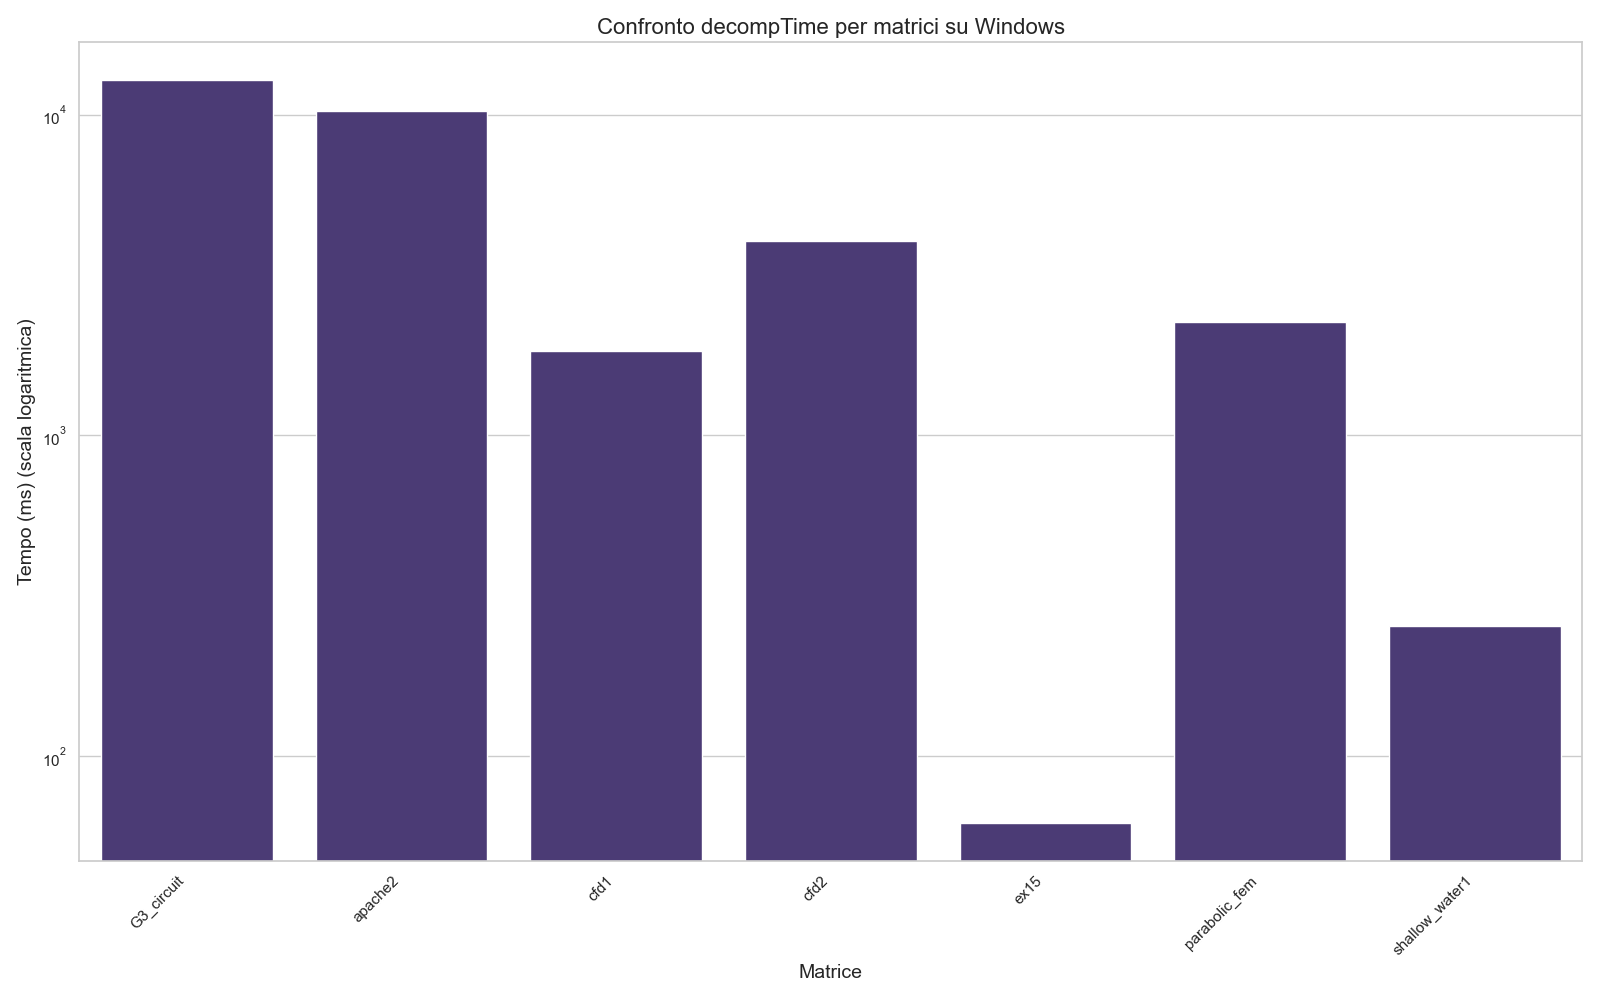
\includegraphics[width=0.9\textwidth]{images/MATLAB/Windows/decompTime_comparison}
    \caption{Confronto dei tempi di decomposizione su Windows MATLAB per diverse matrici (scala logaritmica).}
    \label{fig:matlab-windows-decomp-comparison}
\end{figure}

\begin{figure}[H]
    \centering
    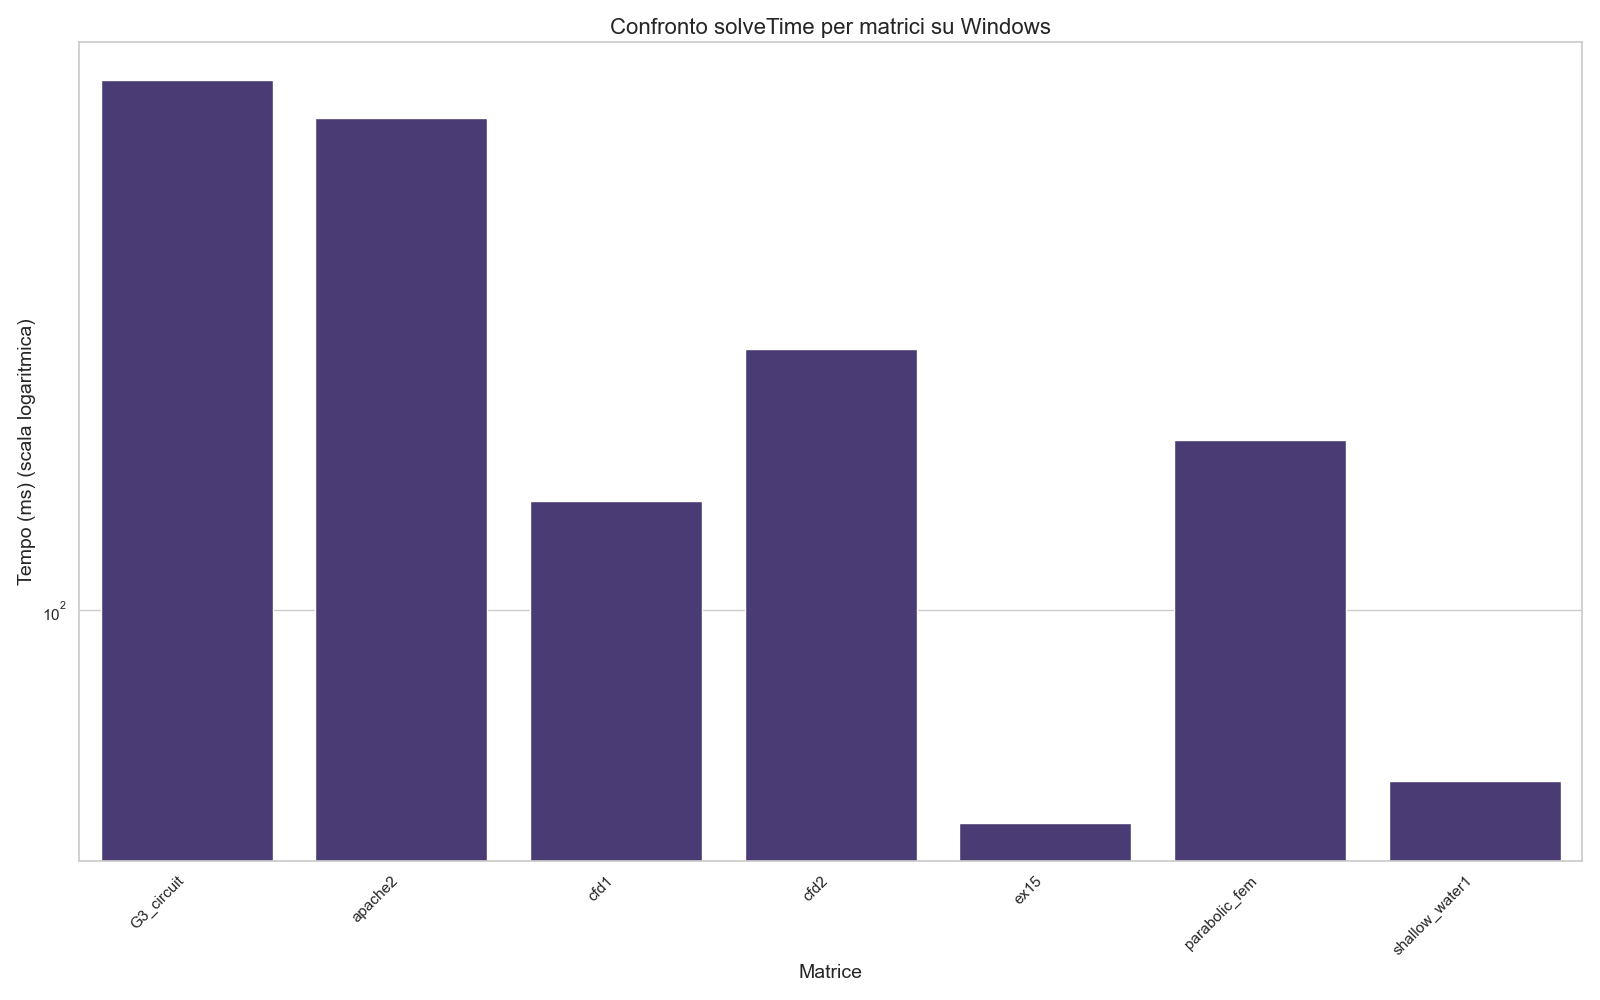
\includegraphics[width=0.9\textwidth]{images/MATLAB/Windows/solveTime_comparison}
    \caption{Confronto dei tempi di risoluzione su Windows MATLAB per diverse matrici (scala logaritmica).}
    \label{fig:matlab-windows-solve-comparison}
\end{figure}

\begin{figure}[H]
    \centering
    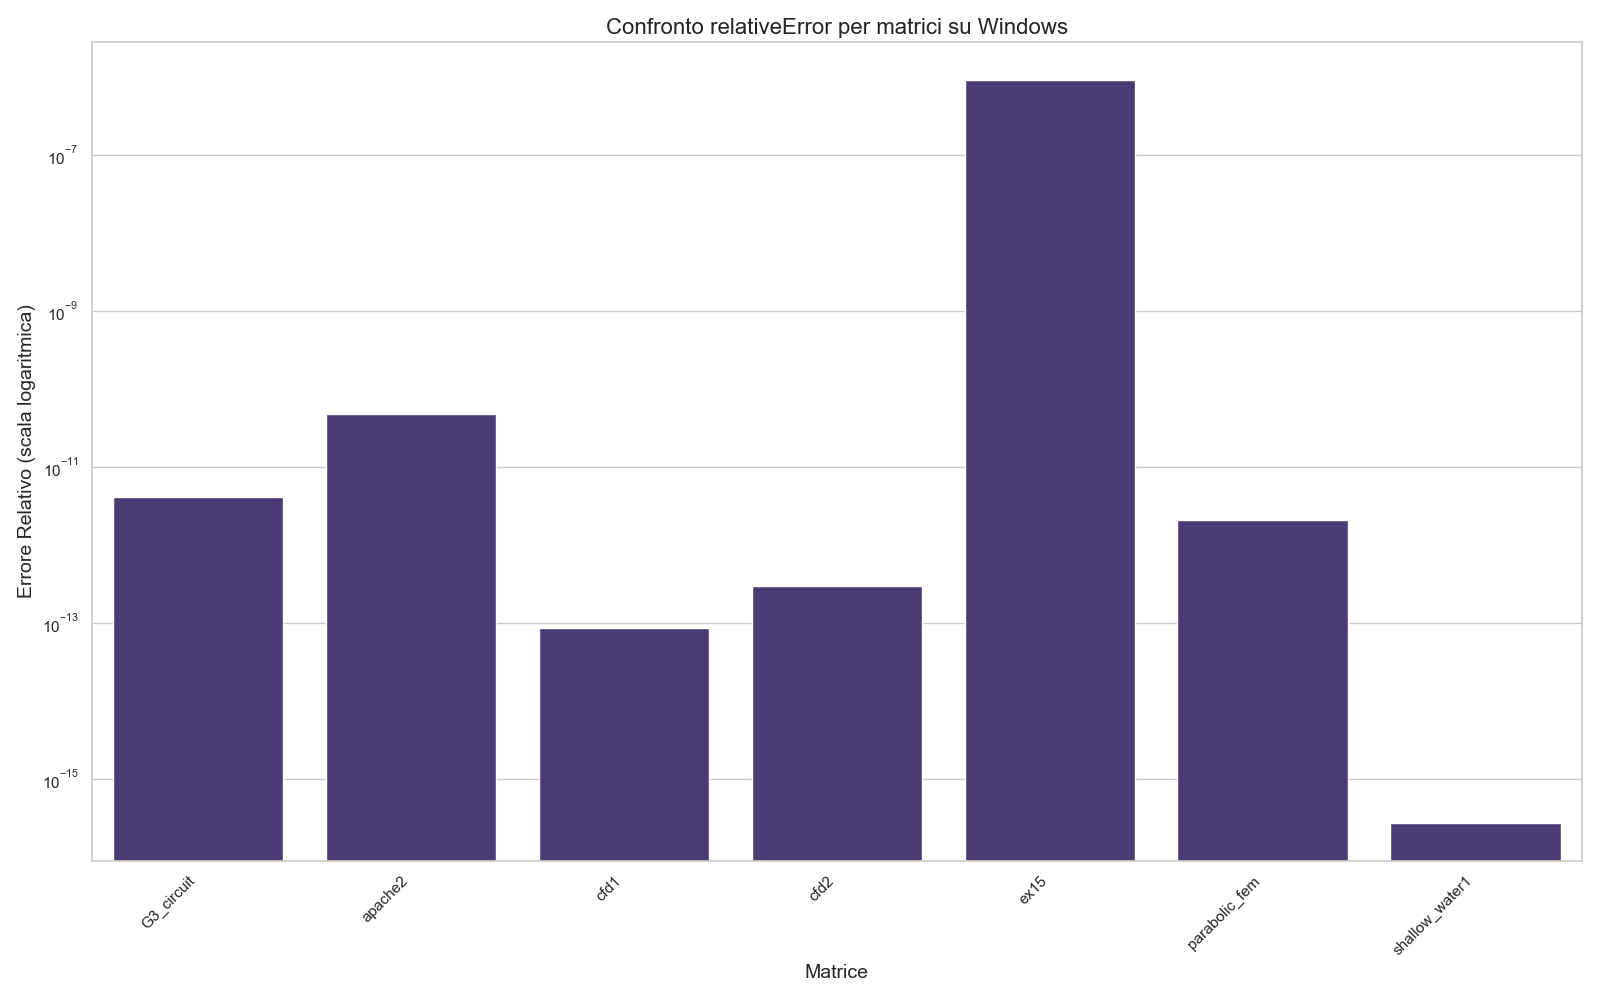
\includegraphics[width=0.9\textwidth]{images/MATLAB/Windows/relativeError_comparison}
    \caption{Confronto dell'errore relativo su Windows MATLAB per diverse matrici (scala logaritmica).}
    \label{fig:matlab-windows-error-comparison}
\end{figure}

\subsection{Linux}

Durante l'esecuzione due matrici hanno causato il kill del processo MATLAB, quindi non sono state incluse nei risultati. Le matrici che hanno causato il crash sono:
\begin{itemize}
    \item Flan\_1565
    \item StocF-1465
\end{itemize}

\begin{figure}[H]
    \centering
    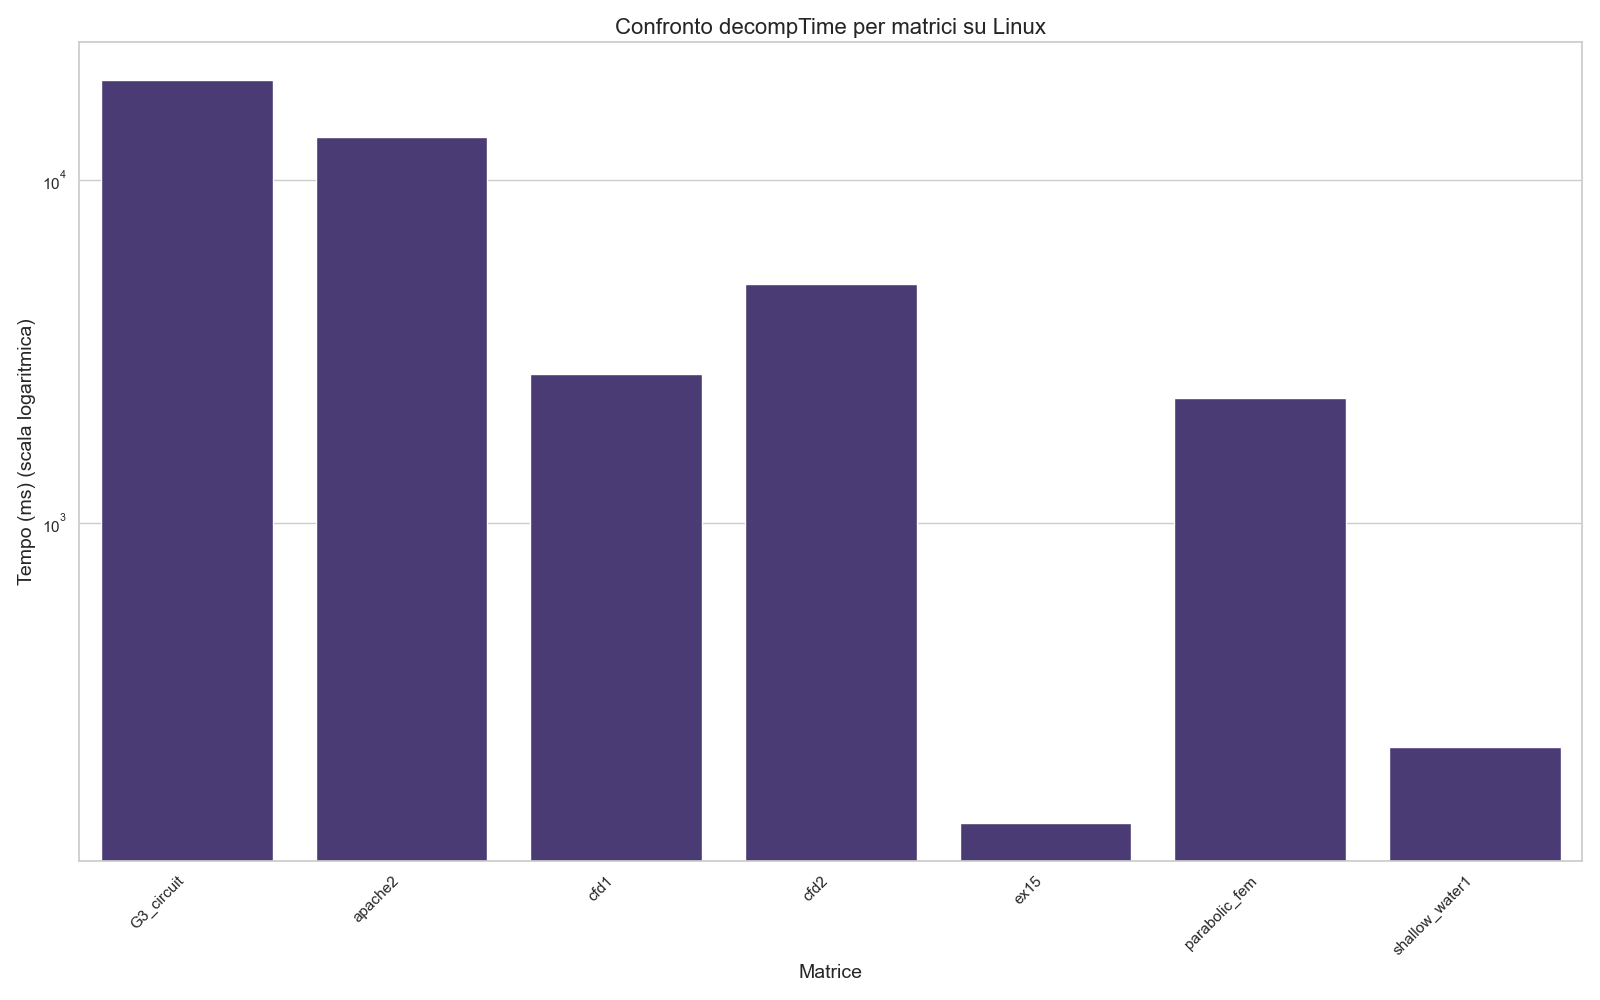
\includegraphics[width=0.9\textwidth]{images/MATLAB/Linux/decompTime_comparison}
    \caption{Confronto dei tempi di decomposizione su Linux MATLAB per diverse matrici (scala logaritmica).}
    \label{fig:matlab-linux-decomp-comparison}
\end{figure}

\begin{figure}[H]
    \centering
    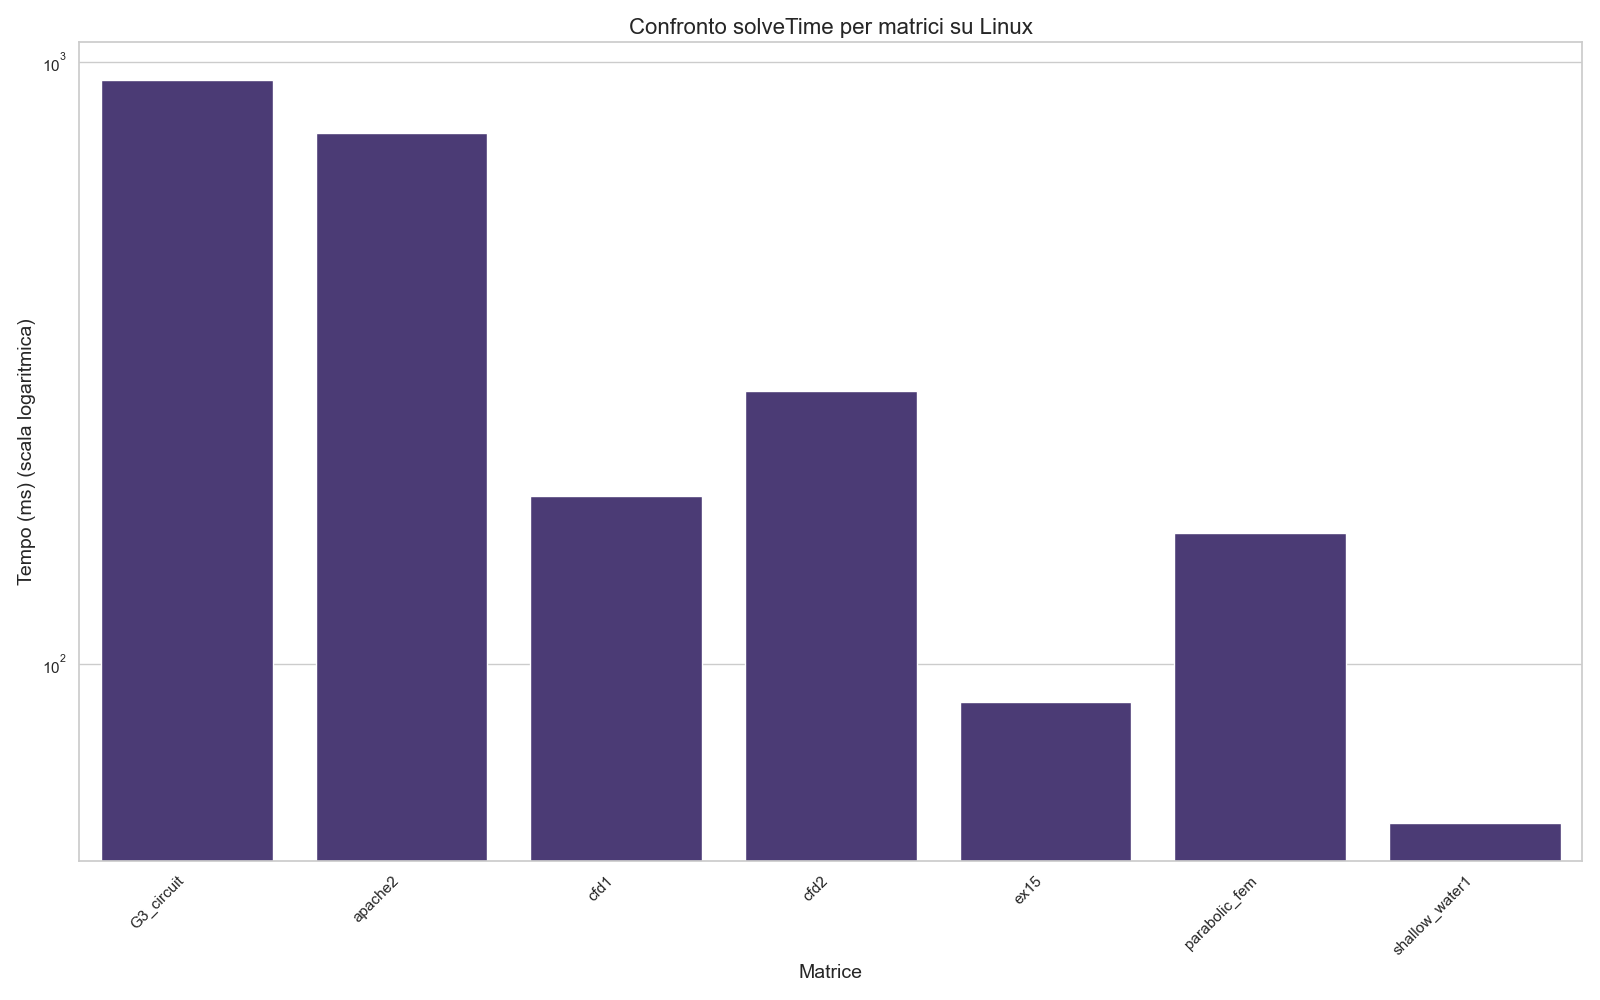
\includegraphics[width=0.9\textwidth]{images/MATLAB/Linux/solveTime_comparison}
    \caption{Confronto dei tempi di risoluzione su Linux MATLAB per diverse matrici (scala logaritmica).}
    \label{fig:matlab-linux-solve-comparison}
\end{figure}

\begin{figure}[H]
    \centering
    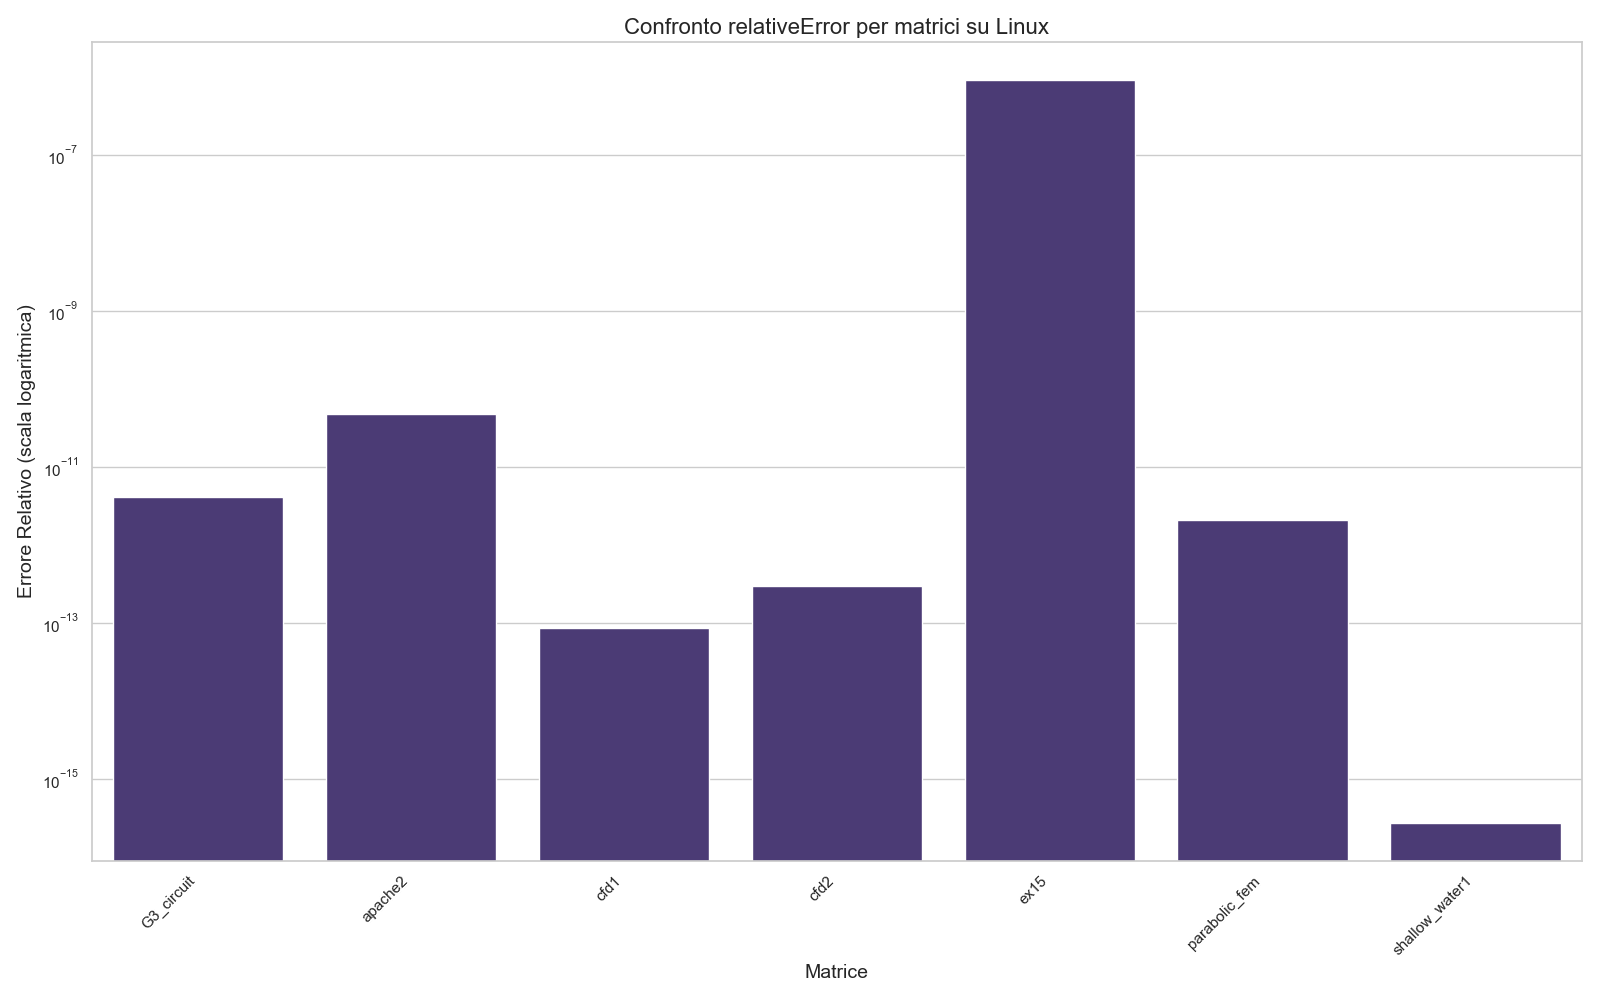
\includegraphics[width=0.9\textwidth]{images/MATLAB/Linux/relativeError_comparison}
    \caption{Confronto dell'errore relativo su Linux MATLAB per diverse matrici (scala logaritmica).}
    \label{fig:matlab-linux-error-comparison}
\end{figure}

\section{Risultati C++}

\subsection{Considerazioni Comuni}

La memoria è la stessa tra i tre sistemi operativi, quindi non è necessario ripeterla per ogni sistema operativo.

\begin{table}[H]
    \centering
    \caption{Memory Usage (MB) for Linux with OpenBLAS}
    \begin{tabular}{lccc}
        \toprule
        Matrix Name & Load Memory (MB) & Decomp Memory (MB) & Solve Memory (MB) \\
        \midrule
        ex15 & \byteToMB{1633680} & \byteToMB{10066112} & \byteToMB{110632} \\
        G3\_circuit & \byteToMB{135257048} & \byteToMB{1864191496} & \byteToMB{25380136} \\
        shallow\_water1 & \byteToMB{5898248} & \byteToMB{71736592} & \byteToMB{1315568} \\
        apache2 & \byteToMB{82807336} & \byteToMB{1819149680} & \byteToMB{11464600} \\
        cfd1 & \byteToMB{29819080} & \byteToMB{347248432} & \byteToMB{1140360} \\
        cfd2 & \byteToMB{50393896} & \byteToMB{609957832} & \byteToMB{1986776} \\
        Flan\_1565 & \byteToMB{1891015064} & \byteToMB{22316964832} & \byteToMB{25083360} \\
        parabolic\_fem & \byteToMB{63000608} & \byteToMB{725188360} & \byteToMB{8421880} \\
        StocF-1465 & \byteToMB{347807328} & \byteToMB{11966096720} & \byteToMB{23497736} \\
        \bottomrule
    \end{tabular}
    \label{tab:memory_usage}
\end{table}

\subsection{Windows}

\begin{figure}[H]
    \centering
    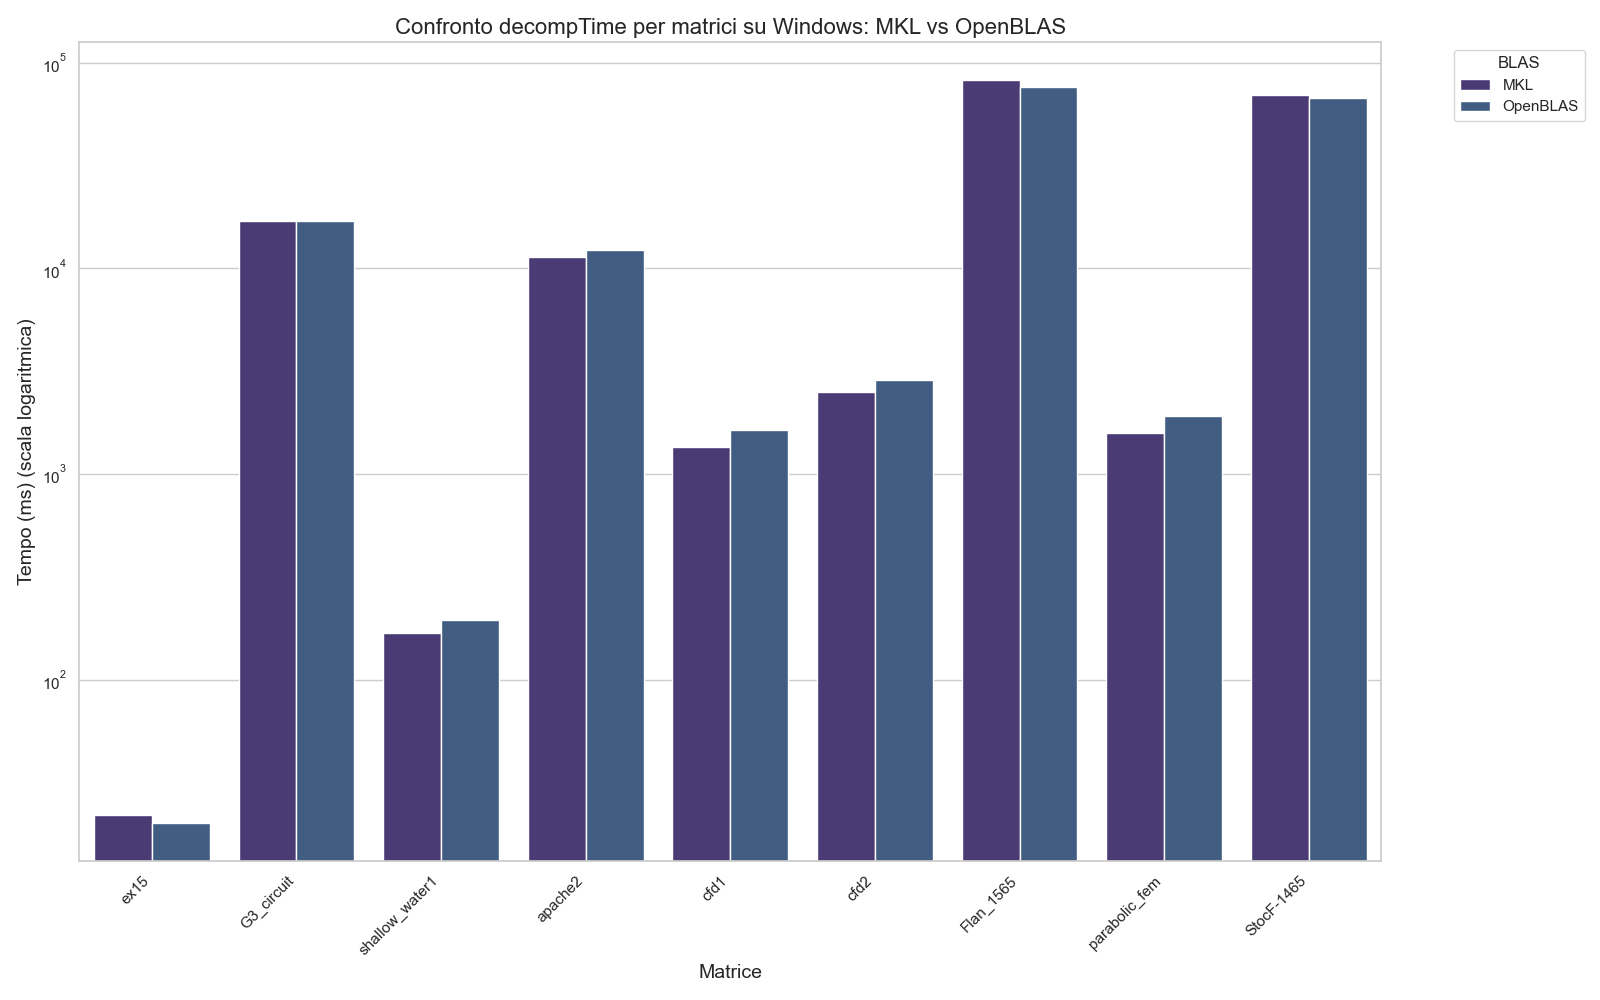
\includegraphics[width=0.9\textwidth]{images/C++/Windows/decompTime_comparison}
    \caption{Confronto dei tempi di decomposizione tra MKL e OpenBLAS su Windows C++ per diverse matrici (scala logaritmica).}
    \label{fig:windows-decomp-comparison}
\end{figure}

\begin{figure}[H]
    \centering
    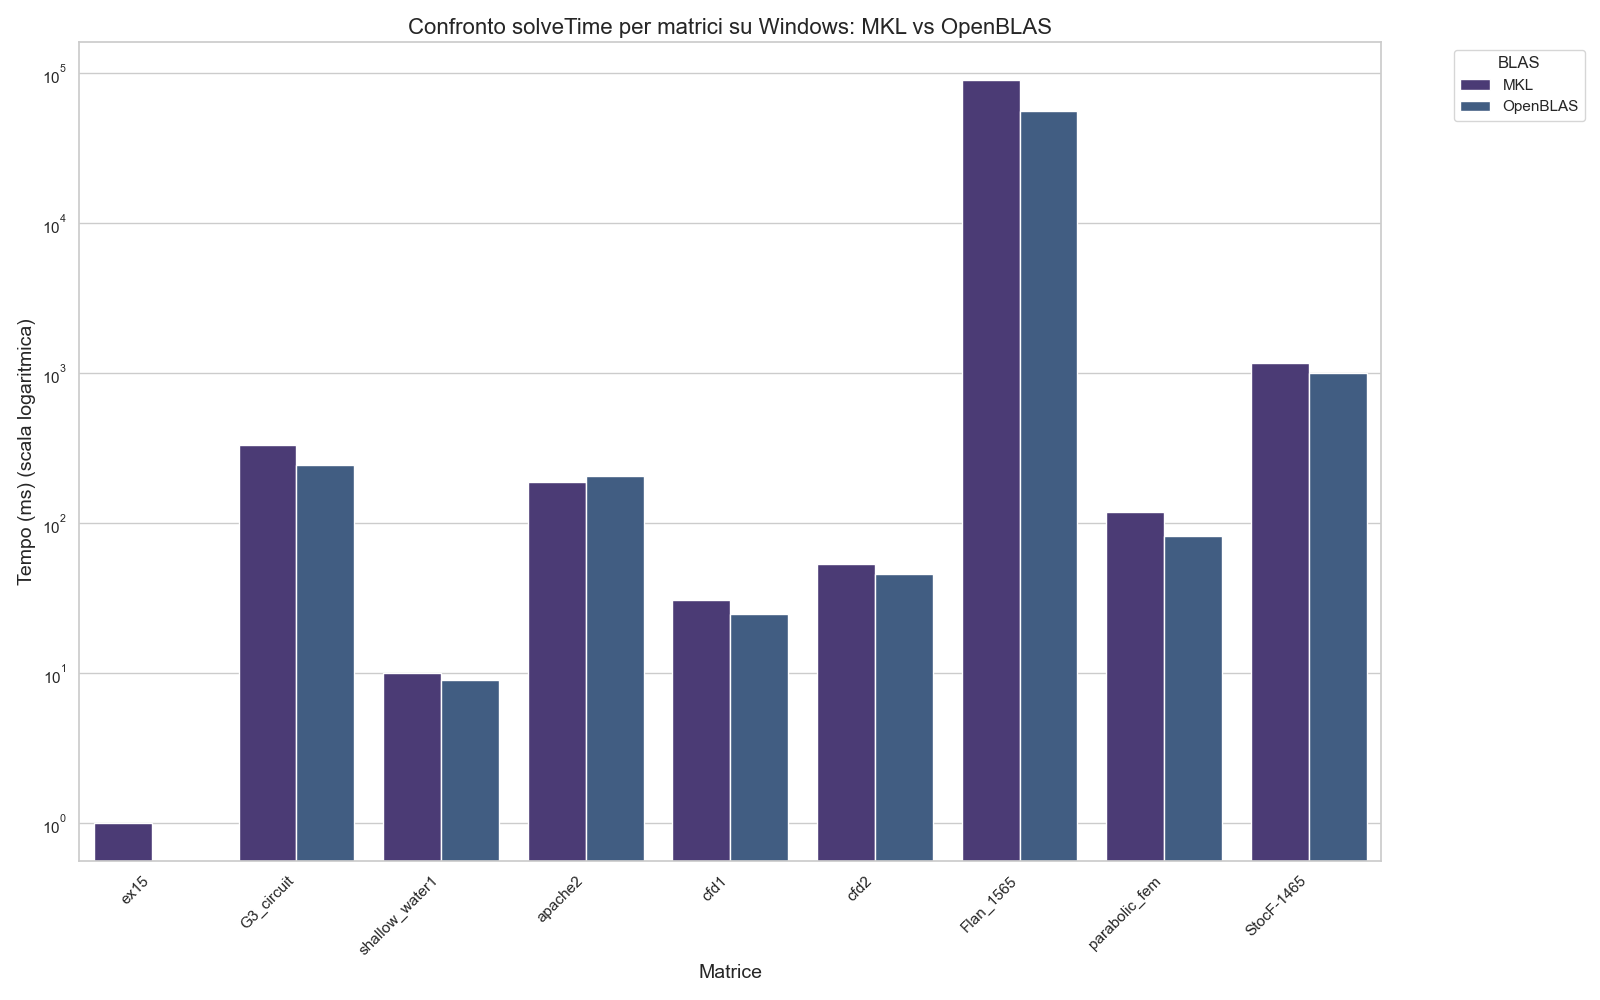
\includegraphics[width=0.9\textwidth]{images/C++/Windows/solveTime_comparison}
    \caption{Confronto dei tempi di risoluzione tra MKL e OpenBLAS su Windows C++ per diverse matrici (scala logaritmica).}
    \label{fig:windows-solve-comparison}
\end{figure}

\begin{figure}[H]
    \centering
    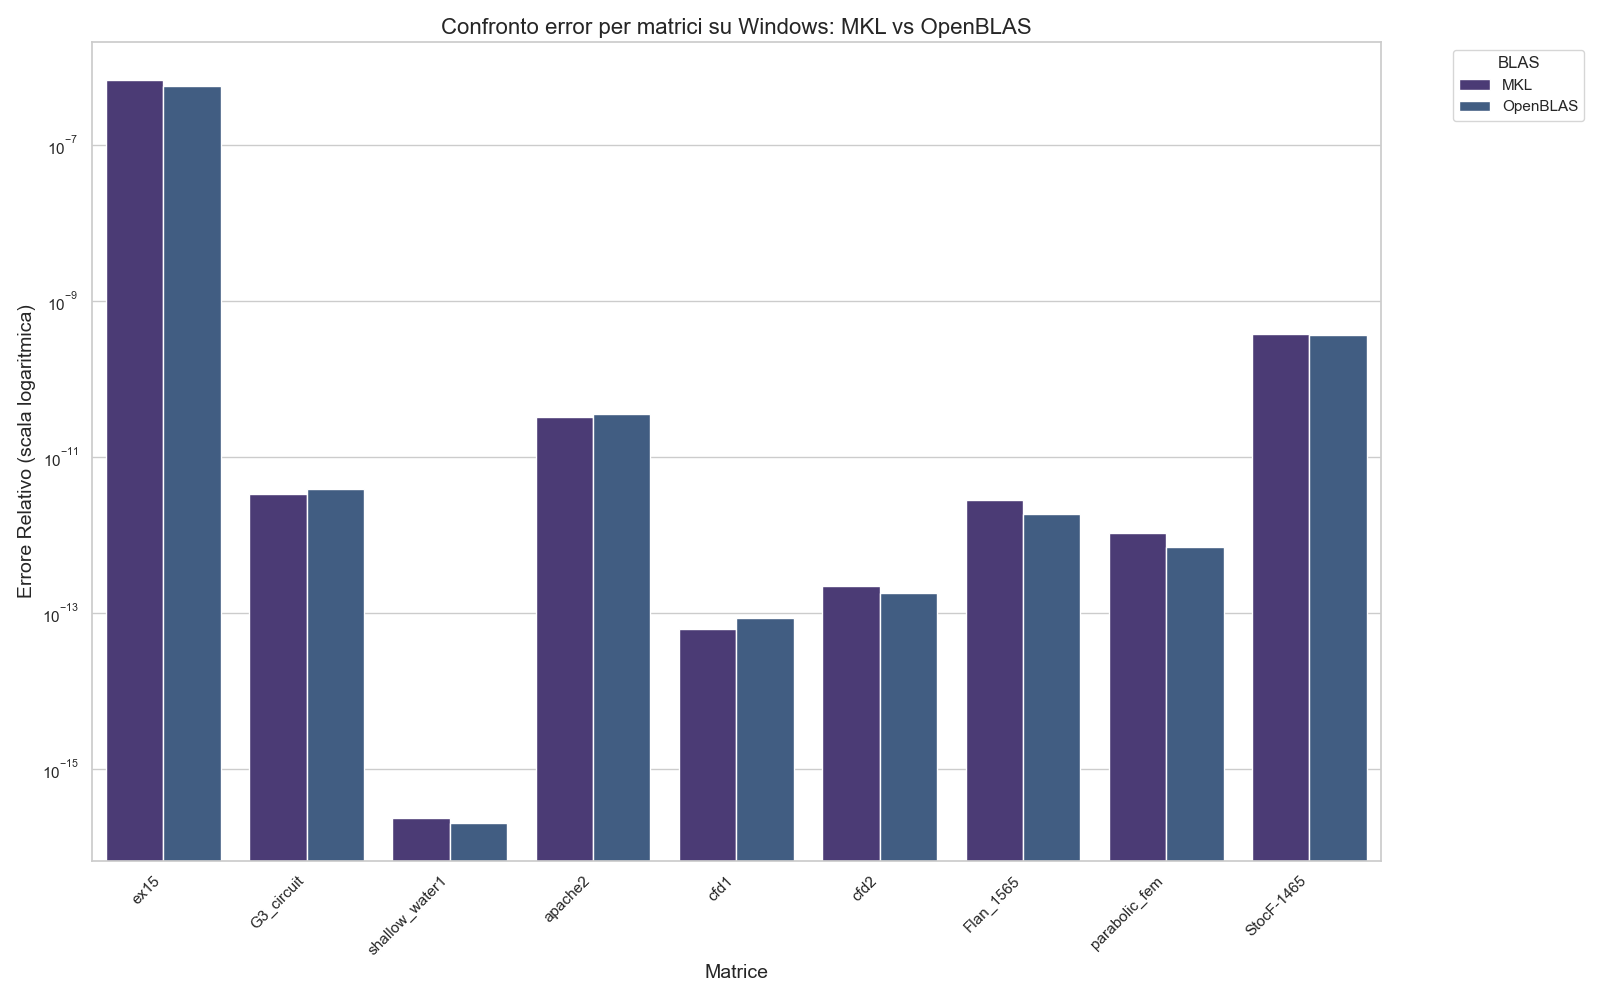
\includegraphics[width=0.9\textwidth]{images/C++/Windows/error_comparison}
    \caption{Confronto dell'errore relativo tra MKL e OpenBLAS su Windows C++ per diverse matrici (scala logaritmica).}
    \label{fig:windows-error-comparison}
\end{figure}

\subsection{Linux}

\begin{figure}[H]
    \centering
    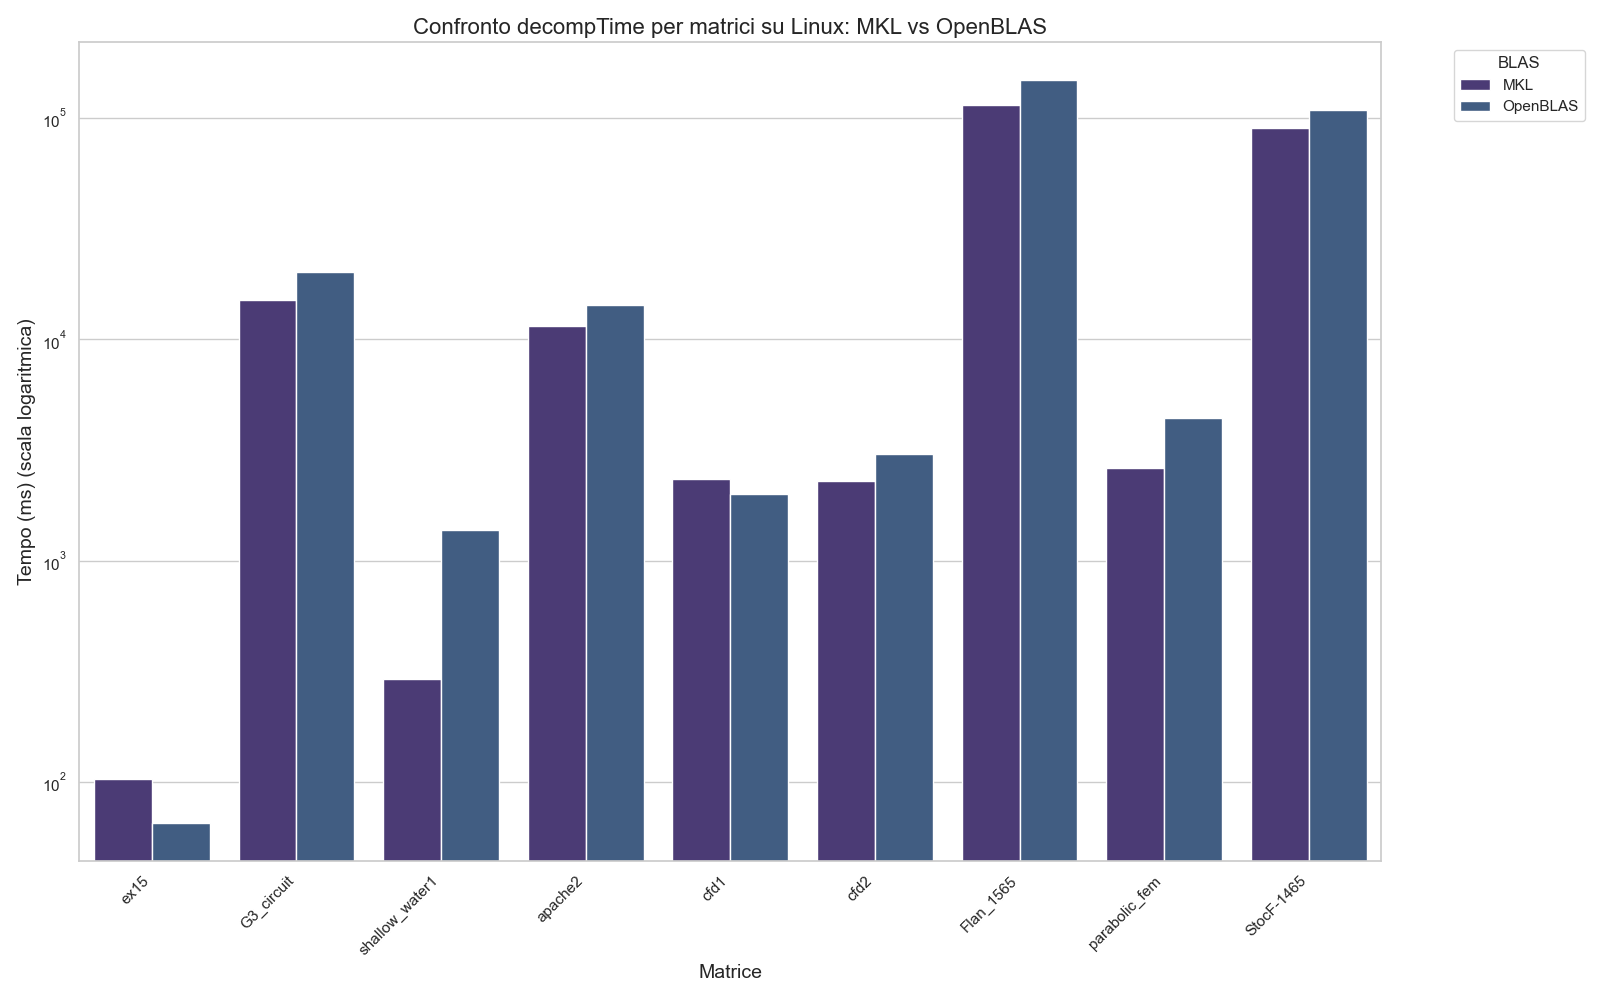
\includegraphics[width=0.9\textwidth]{images/C++/Linux/decompTime_comparison}
    \caption{Confronto dei tempi di decomposizione tra MKL e OpenBLAS su Linux C++ per diverse matrici (scala logaritmica).}
    \label{fig:linux-decomp-comparison}
\end{figure}

\begin{figure}[H]
    \centering
    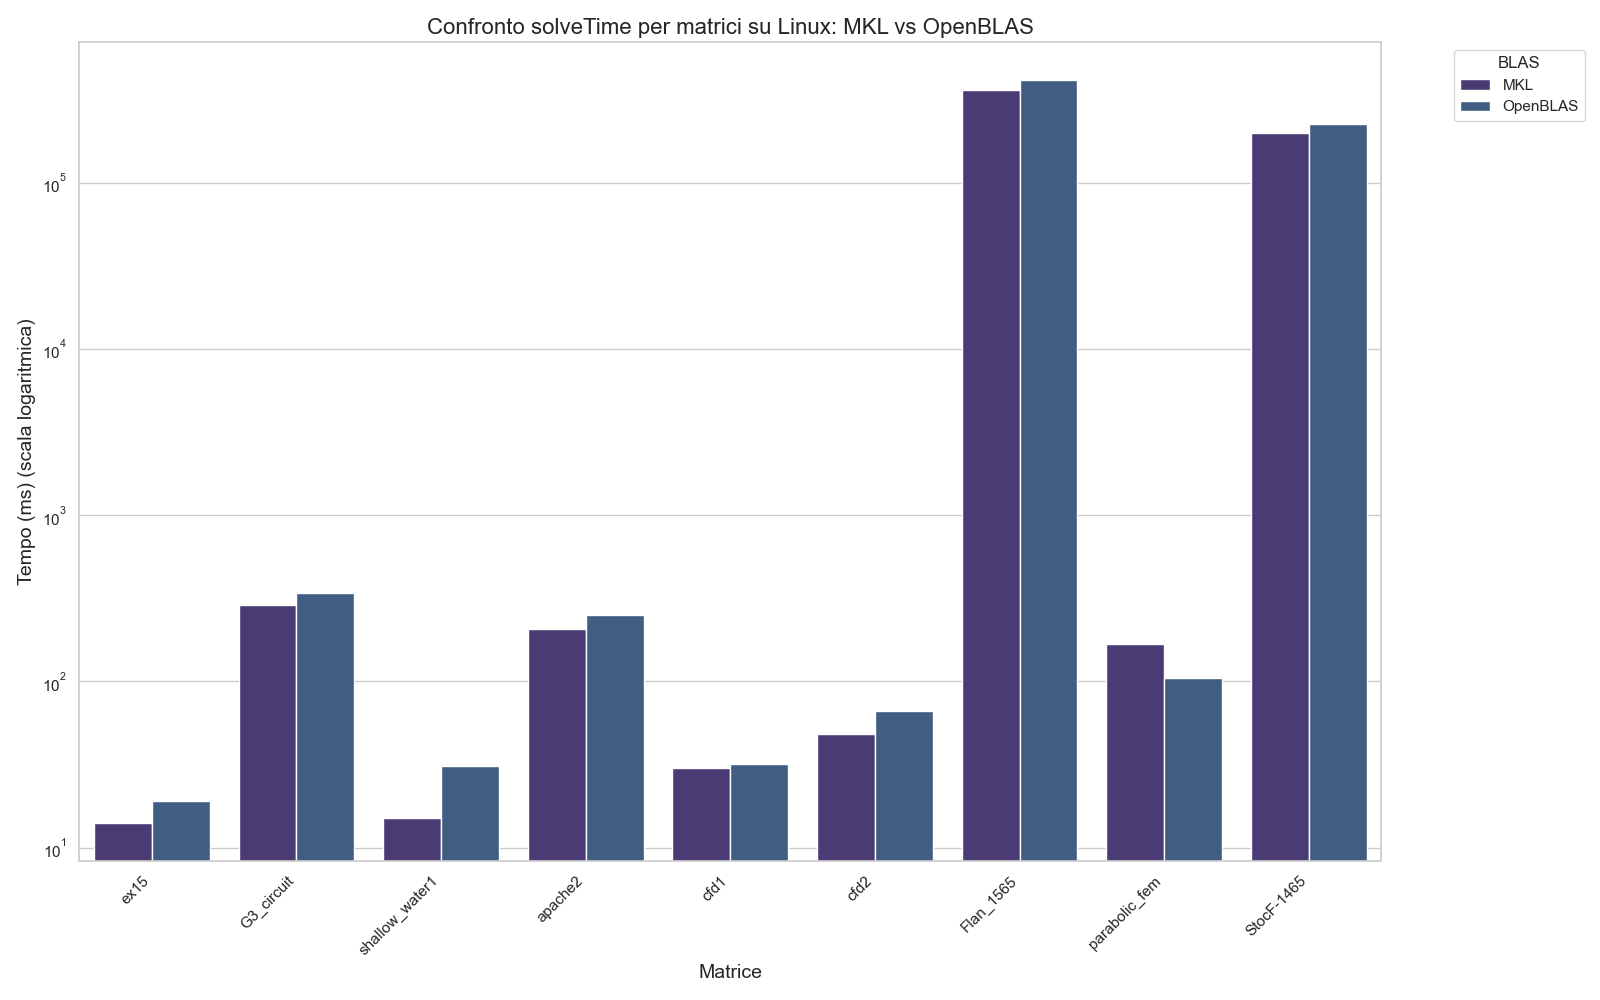
\includegraphics[width=0.9\textwidth]{images/C++/Linux/solveTime_comparison}
    \caption{Confronto dei tempi di risoluzione tra MKL e OpenBLAS su Linux C++ per diverse matrici (scala logaritmica).}
    \label{fig:linux-solve-comparison}
\end{figure}

\begin{figure}[H]
    \centering
    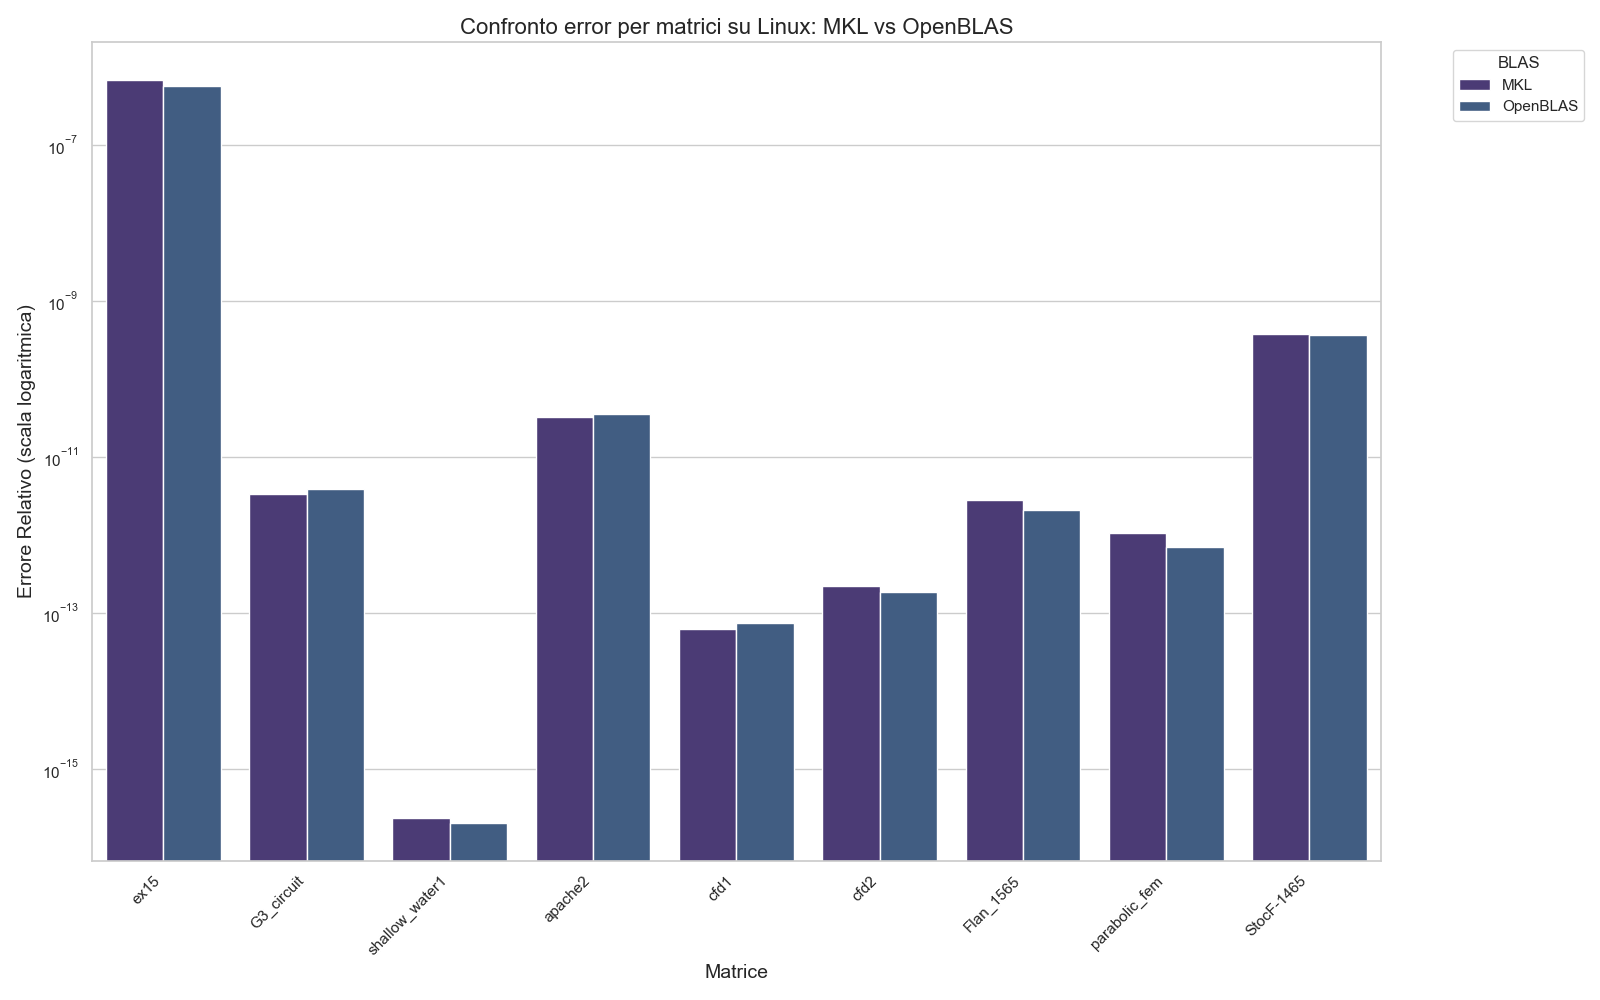
\includegraphics[width=0.9\textwidth]{images/C++/Linux/error_comparison}
    \caption{Confronto dell'errore relativo tra MKL e OpenBLAS su Linux C++ per diverse matrici (scala logaritmica).}
    \label{fig:linux-error-comparison}
\end{figure}

\subsection{MacOS}

\begin{figure}[H]
    \centering
    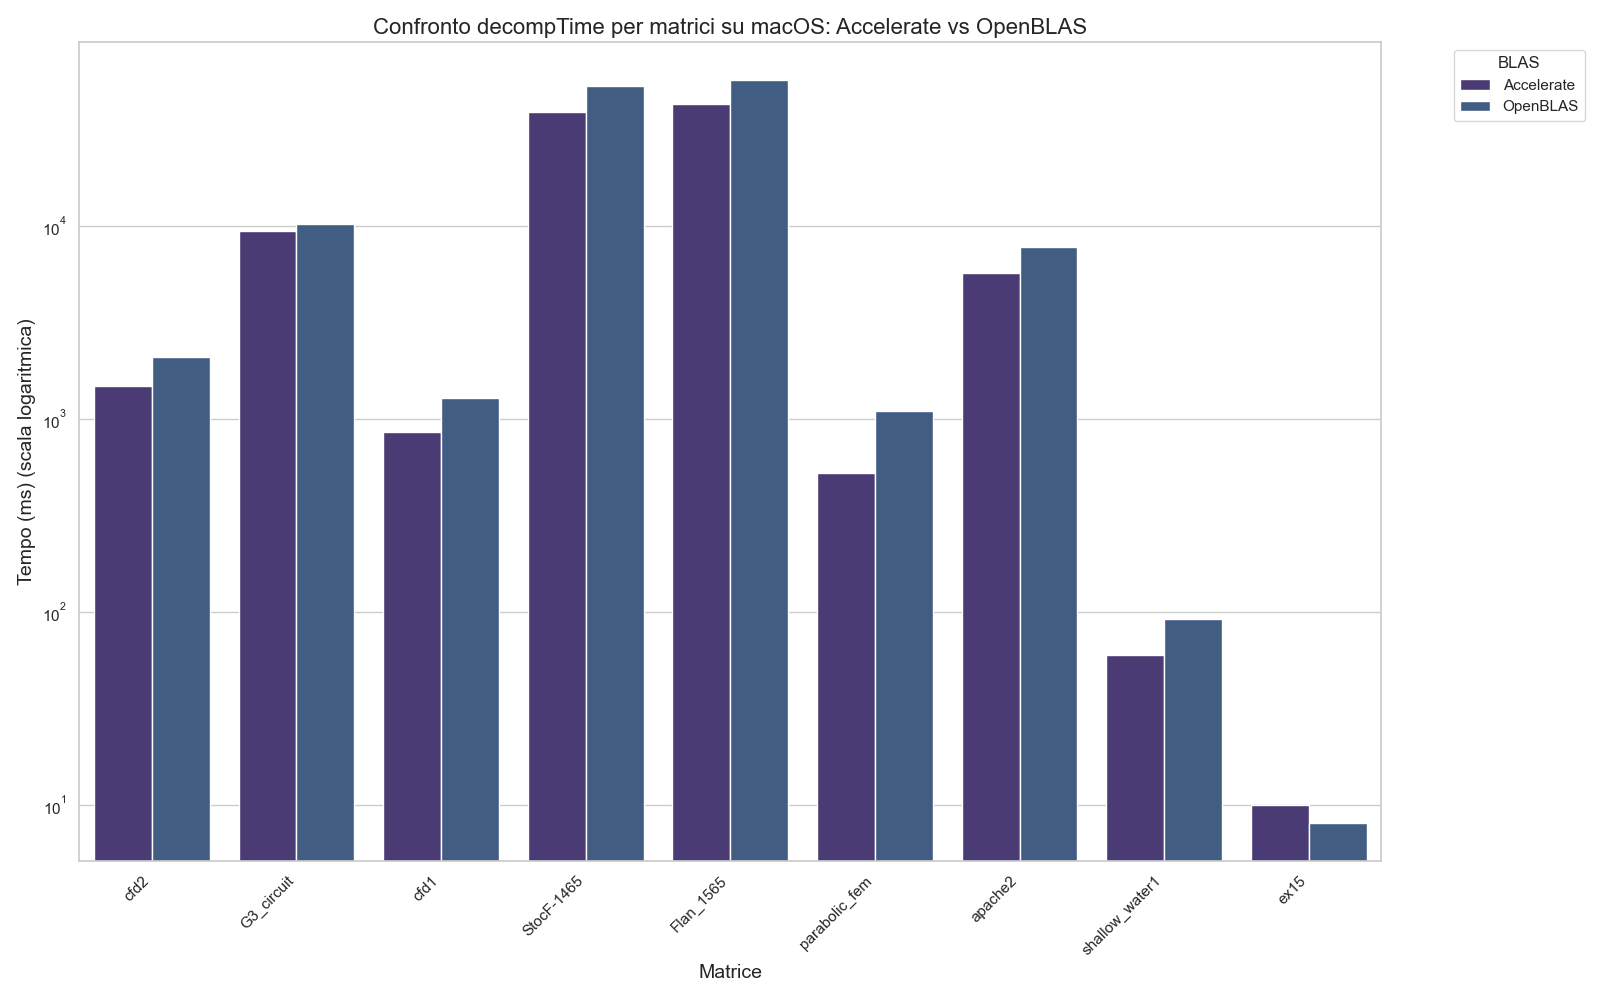
\includegraphics[width=0.9\textwidth]{images/C++/macOs/decompTime_comparison}
    \caption{Confronto dei tempi di decomposizione tra Accelerate e OpenBLAS su MacOS C++ per diverse matrici (scala logaritmica).}
    \label{fig:macos-decomp-comparison}
\end{figure}

\begin{figure}[H]
    \centering
    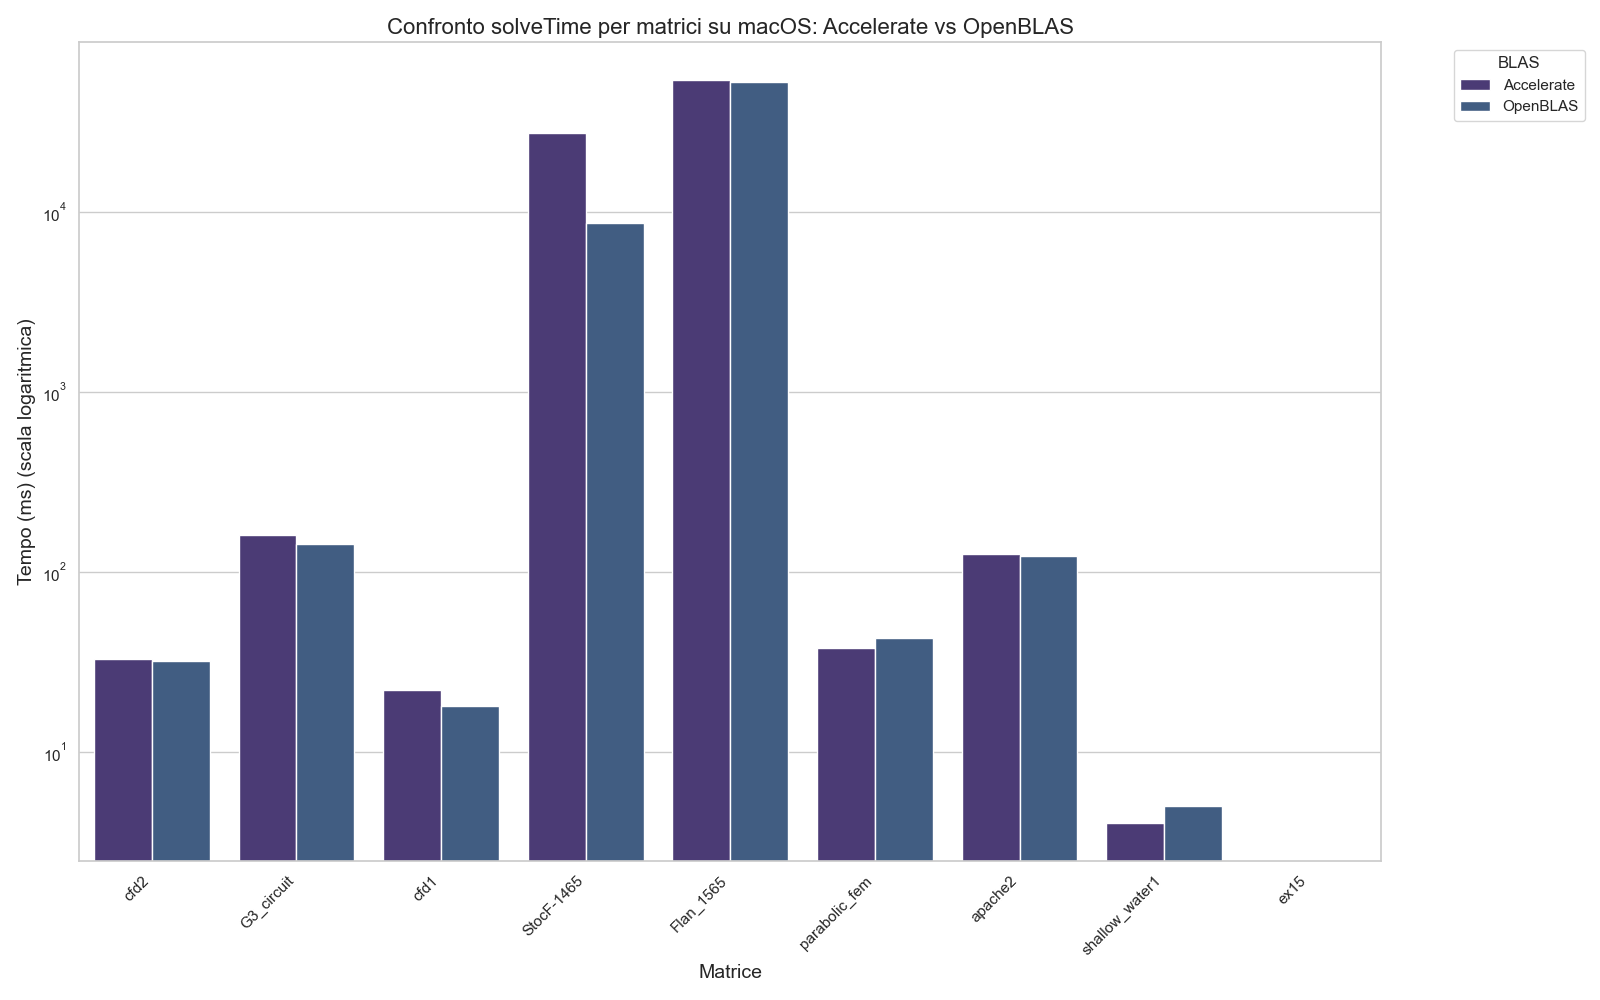
\includegraphics[width=0.9\textwidth]{images/C++/macOs/solveTime_comparison}
    \caption{Confronto dei tempi di risoluzione tra Accelerate e OpenBLAS su MacOS C++ per diverse matrici (scala logaritmica).}
    \label{fig:macos-solve-comparison}
\end{figure}

\begin{figure}[H]
    \centering
    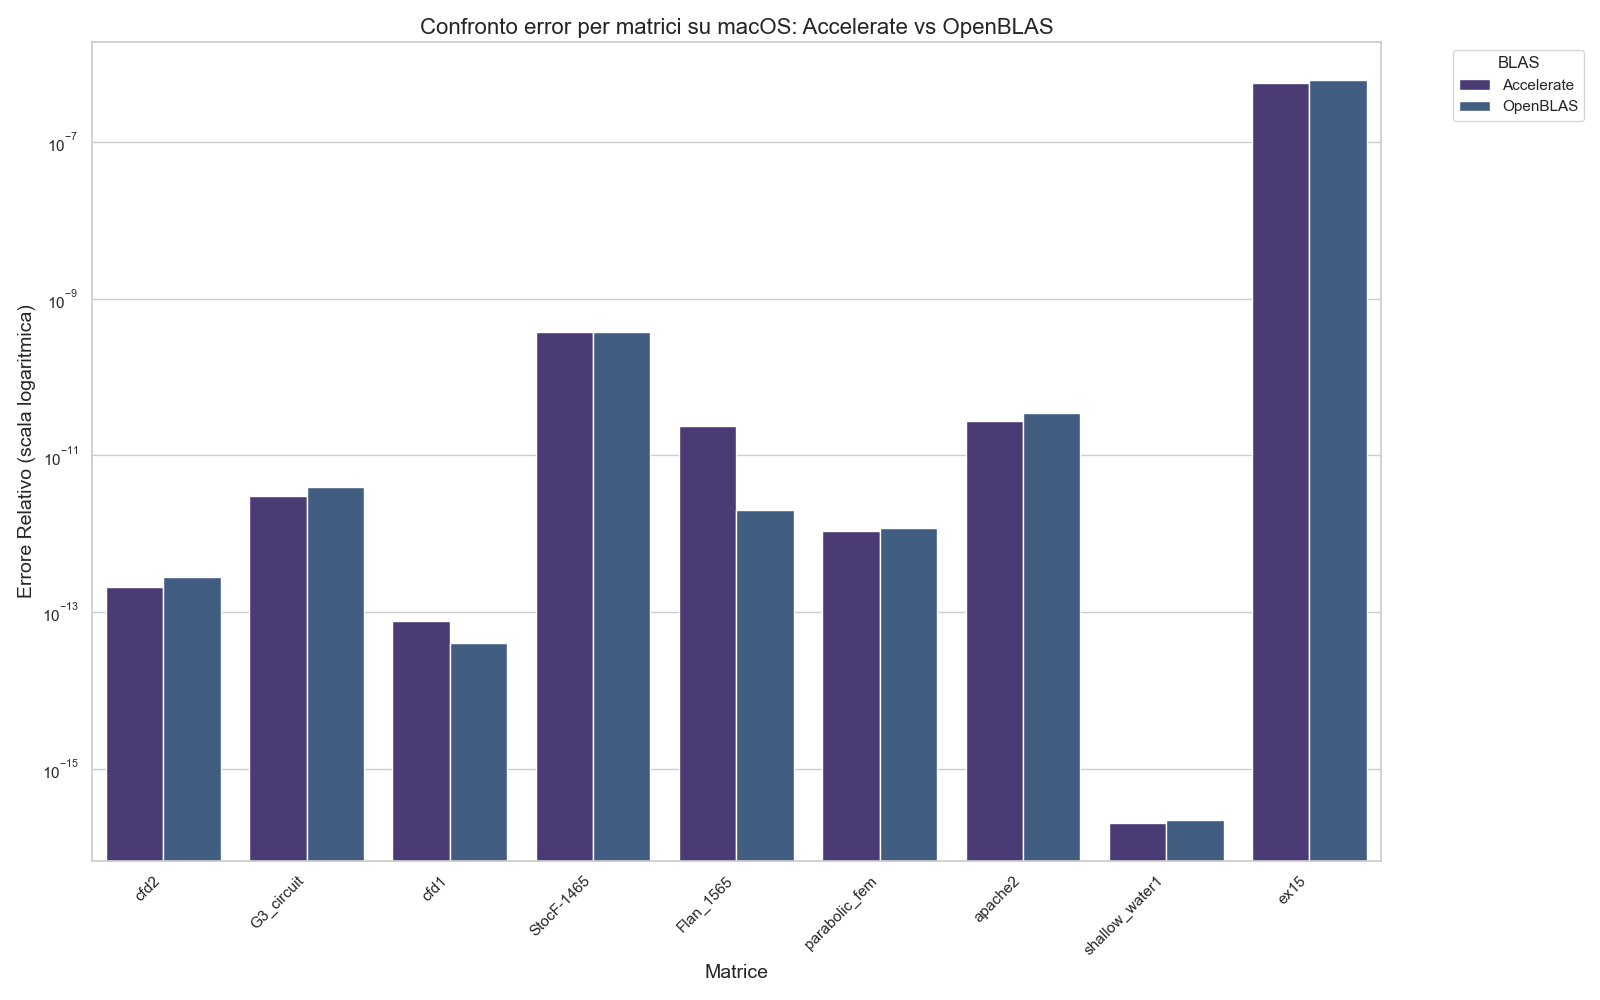
\includegraphics[width=0.9\textwidth]{images/C++/macOs/error_comparison}
    \caption{Confronto dell'errore relativo tra Accelerate e OpenBLAS su MacOS C++ per diverse matrici (scala logaritmica).}
    \label{fig:macos-error-comparison}
\end{figure}

\subsection{Riepilogo dei risultati}

\begin{figure}[H]
    \centering
    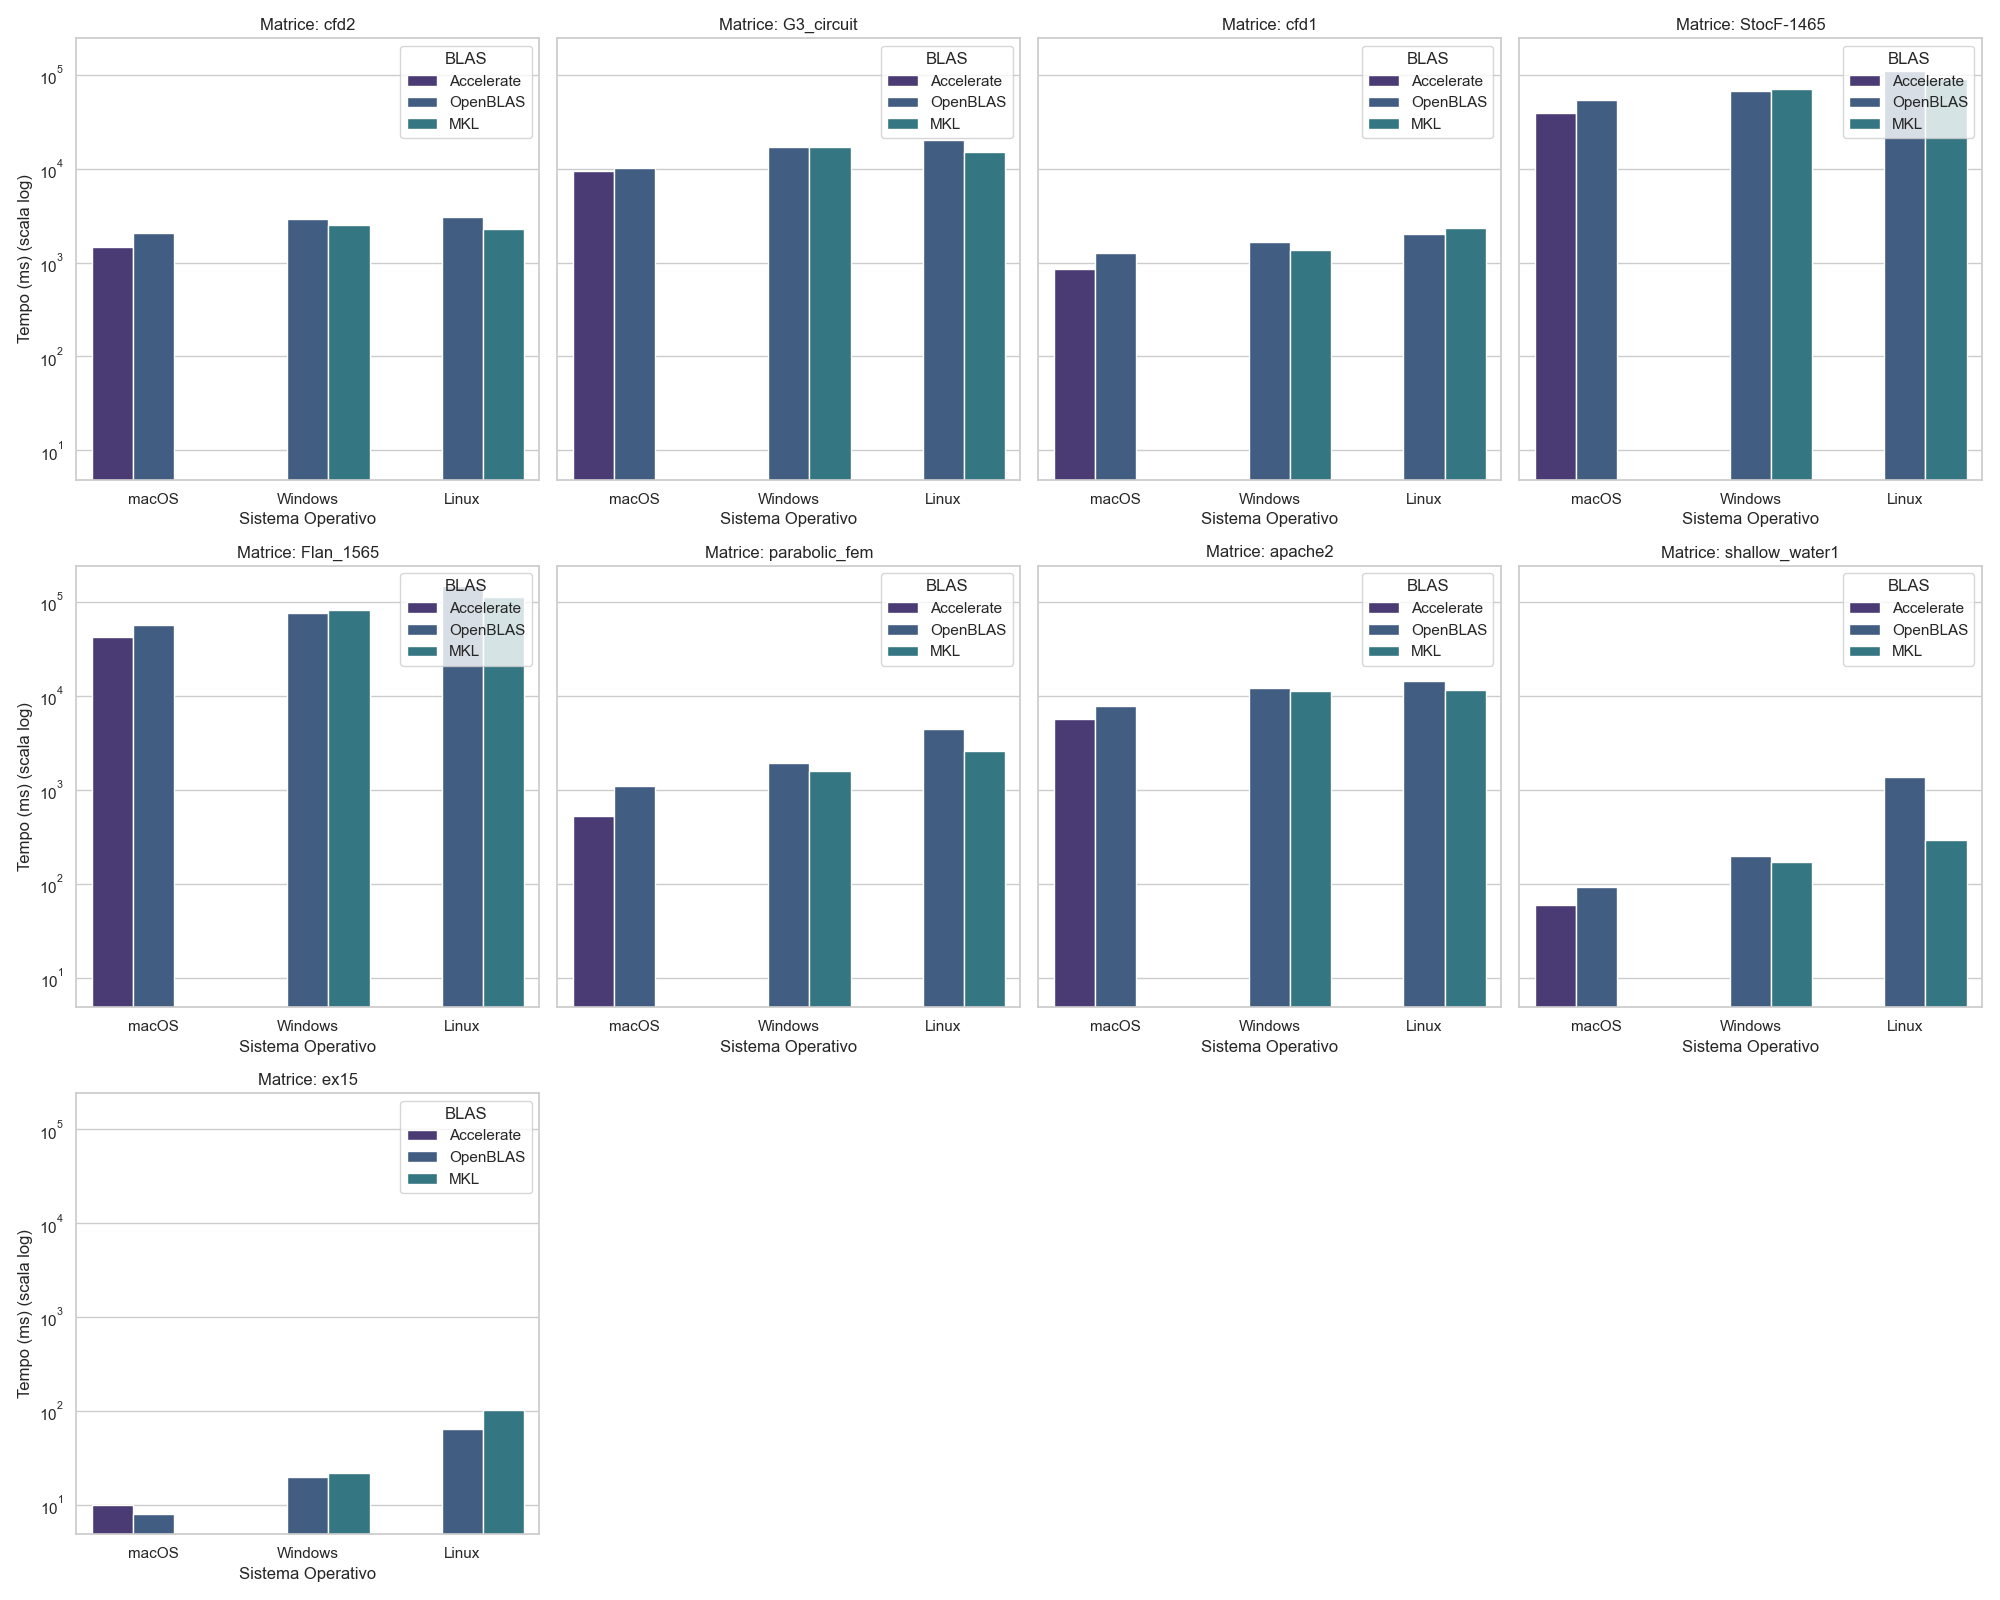
\includegraphics[width=0.9\textwidth]{images/C++/decompTime_facet_grid}
    \caption{Confronto dei tempi di decomposizione tra MKL e OpenBLAS su C++ per diverse matrici (scala logaritmica).}
    \label{fig:decomp-comparison}
\end{figure}

\begin{figure}[H]
    \centering
    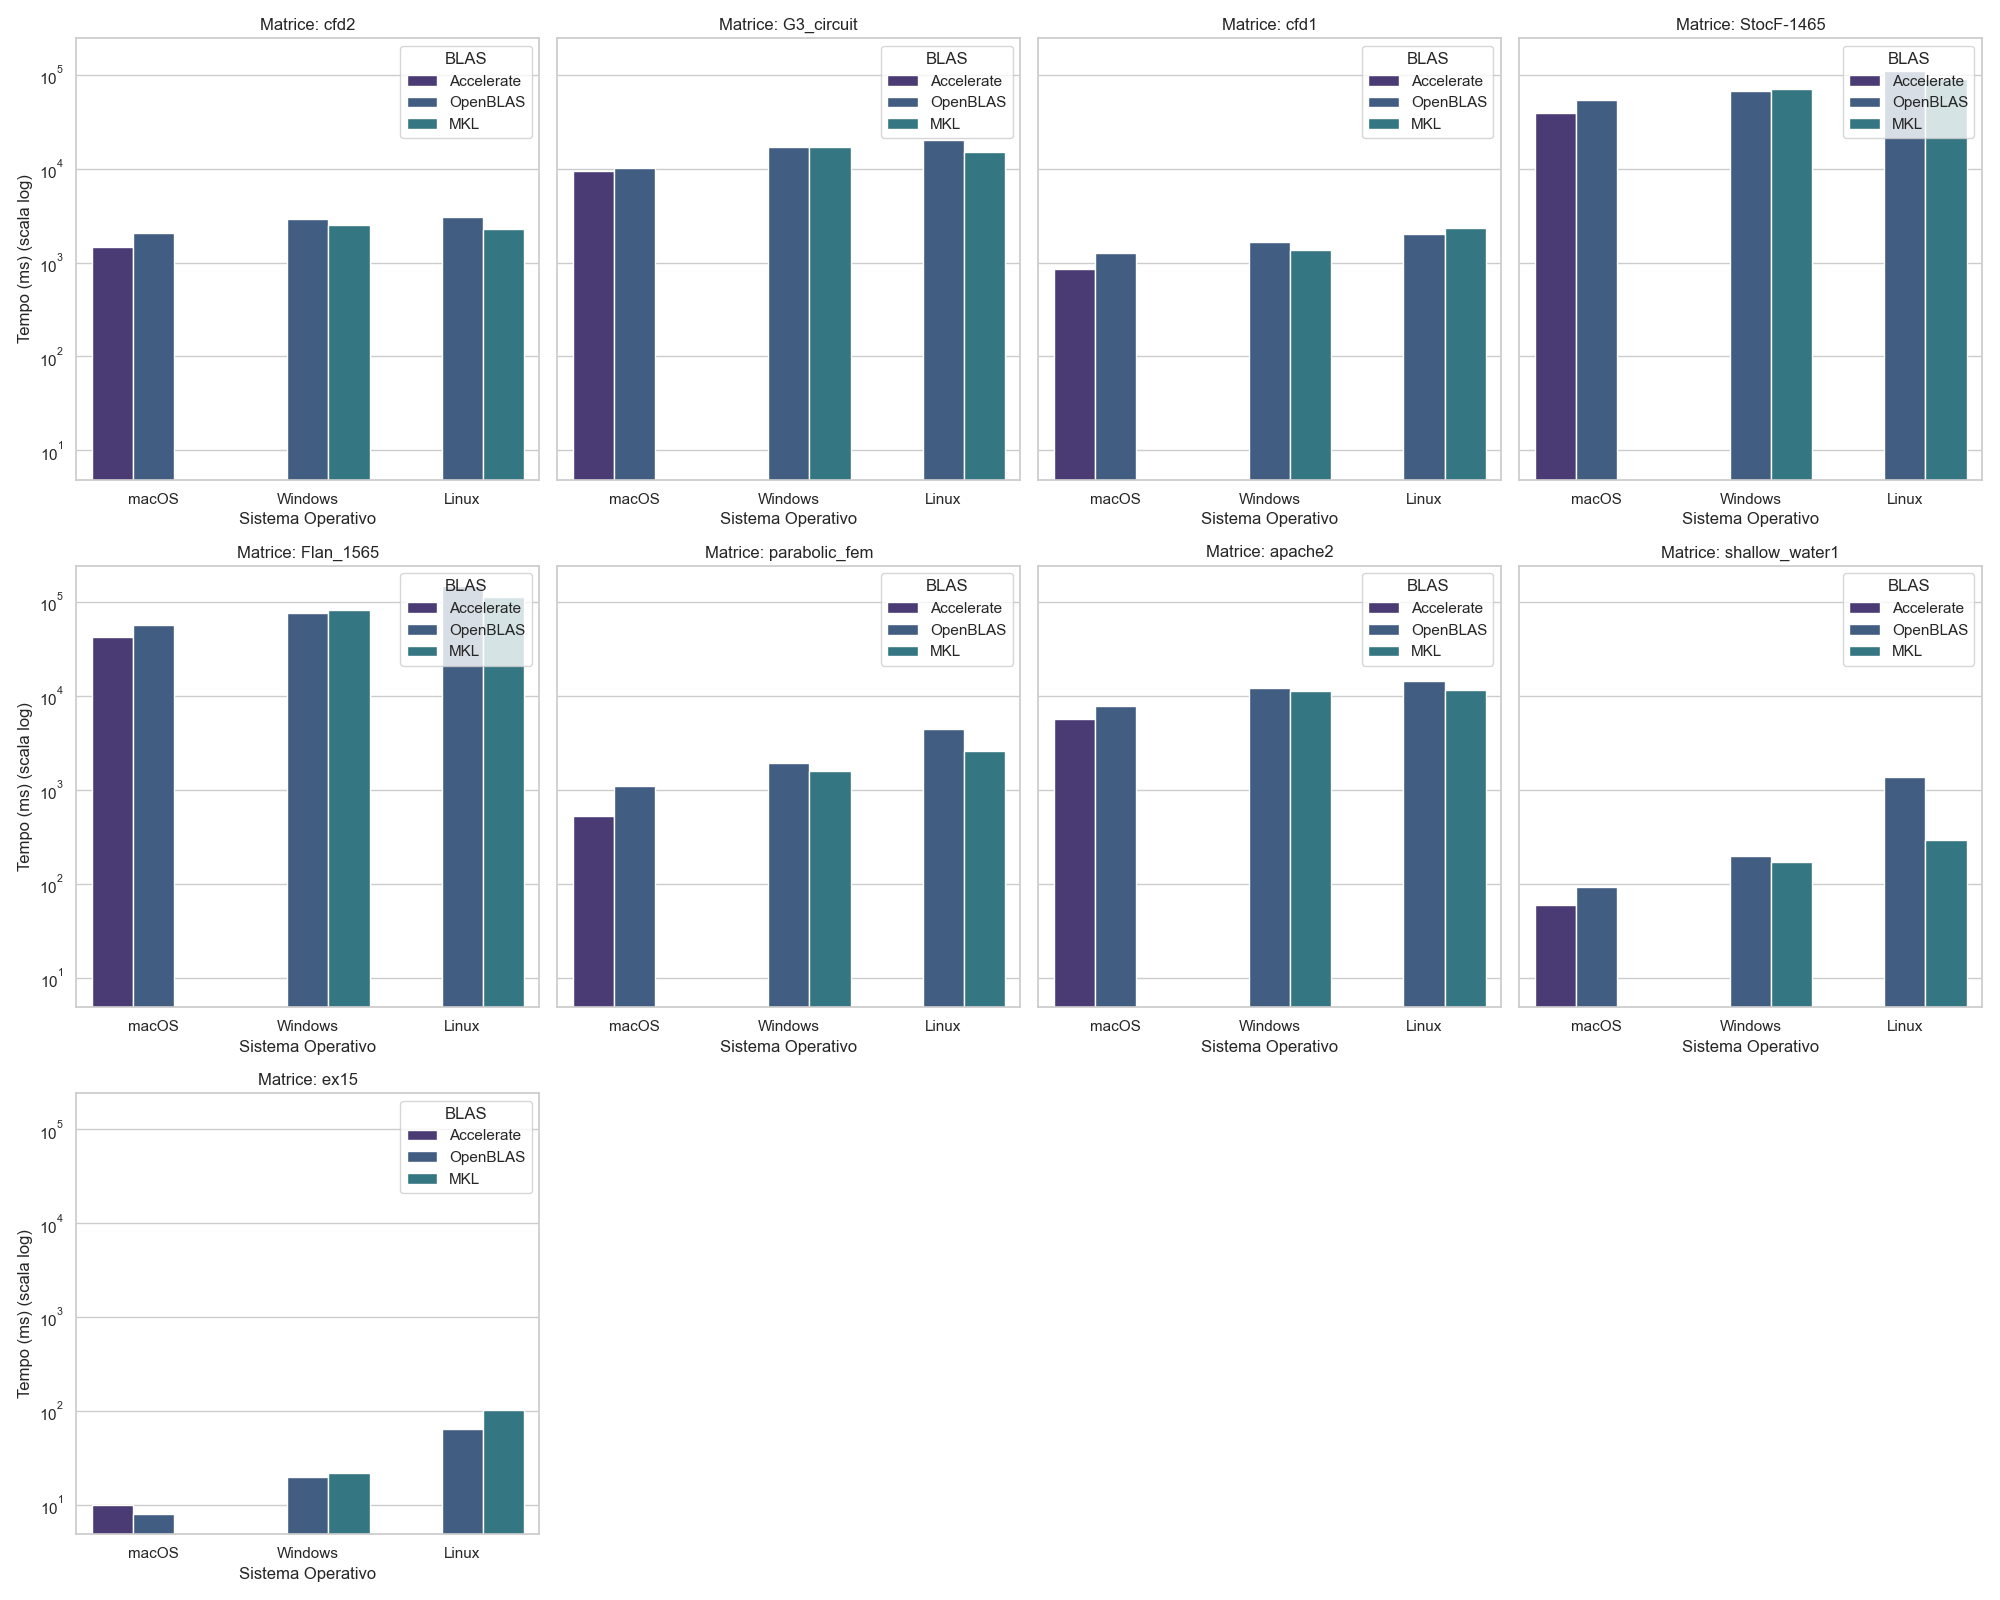
\includegraphics[width=0.9\textwidth]{images/C++/decompTime_facet_grid}
    \caption{Confronto dei tempi di decomposizione tra MKL e OpenBLAS su C++ per diverse matrici (scala logaritmica).}
    \label{fig:solve-comparison}
\end{figure}

\begin{figure}[H]
    \centering
    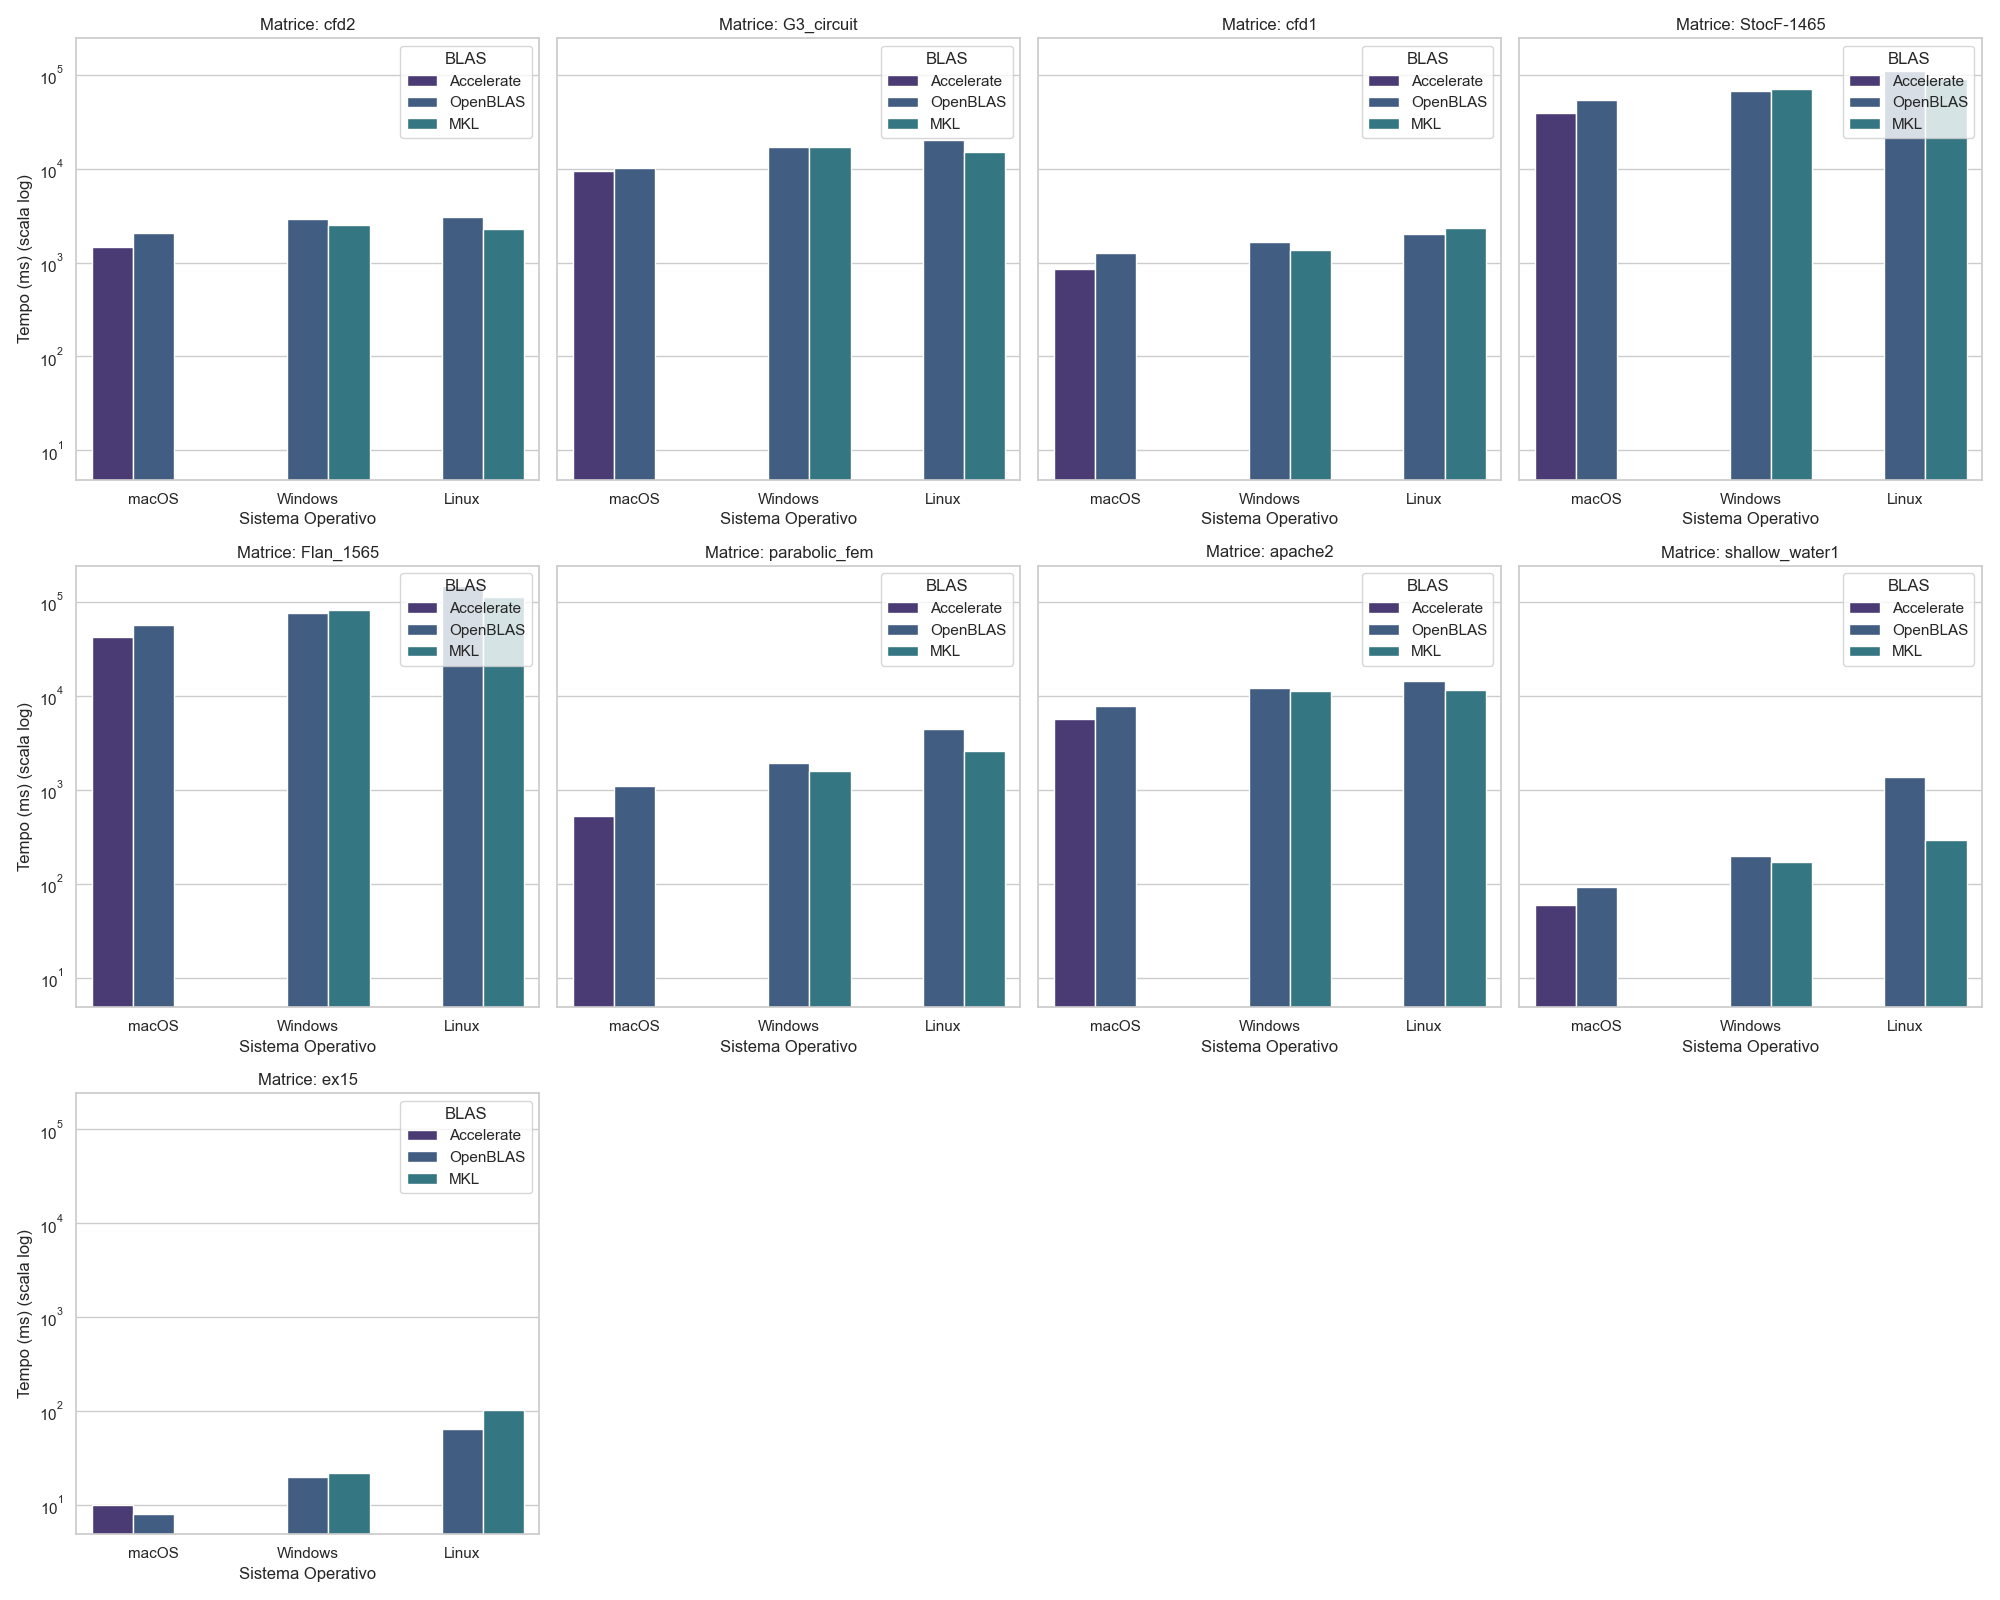
\includegraphics[width=0.9\textwidth]{images/C++/decompTime_facet_grid}
    \caption{Confronto dei tempi di decomposizione tra MKL e OpenBLAS su C++ per diverse matrici (scala logaritmica).}
    \label{fig:error-comparison}
\end{figure}
